% press command+option+B to build, or change "Auto Build: Run" in Settings.

\documentclass{book}

\usepackage{xeCJK}
\usepackage{geometry}
\usepackage{titlesec}

\usepackage{underlin}
\usepackage{wrapfig}
\usepackage{caption}
\usepackage{graphicx}
\usepackage{pdfpages}
\usepackage{multirow}%表格合并行列单元格

% 分栏并浮动图片
\usepackage{float}
\usepackage{multicol}
\usepackage[none]{hyphenat}
\usepackage{appendix}

% 数学
\usepackage{unicode-math}%正体希腊字母
\usepackage{mathrsfs}
\usepackage{amsfonts}
\usepackage{bm}
\usepackage{bbm}
% \usepackage{amsmath}
% \usepackage{amssymb}

% 设置图书版式
\usepackage{marginnote}%侧栏
\usepackage{fancyhdr}%页眉页脚页码
\usepackage{indentfirst}%首段空两格
\usepackage{mdframed}%加阴影
\usepackage{color}%特殊字体颜色
\usepackage{setspace}%行距

\usepackage{hyperref}%所有网页用超链接同步挂靠
\usepackage{xpatch}%设置verbatim前后间距

%行号
\usepackage{lineno}

%圆角边框
\usepackage{fancybox}

\def\codereplace#1{%代码中的可替换部分
    \xeCJKsetup{CJKecglue={\hskip 0pt}}
    \textsl{⟨#1⟩}}

\def\wz#1{%网址
    {\ttfamily #1}}

\def\jz#1{%原书脚注
    \footnote{#1}
}

\def\yz#1{%译注
    \footnote{\textsl{译注:}#1}
}

\def\dm#1{%代码
    \texttt{#1}}

\def\dmh#1{%代码行
    {\xeCJKsetup{CJKecglue={\hskip 0pt}}
    \char"258E \texttt{#1}}
}

\def\celan#1{%侧栏TODO三角形方向
$\blacktriangleright$
\marginpar{
        $\blacktriangleleft$\textsf{#1}
    }
}

\definecolor{LightPink}{RGB}{230,173,173}
\newenvironment{exclamation}[1][!]%原书的圆圈感叹号
{
    \begin{mdframed}[backgroundcolor=LightPink,hidealllines=true]
        {\textcircled{\scriptsize #1}} \quad
        \sffamily
}{      
    \rmfamily
    \end{mdframed}
}

\definecolor{LightBlue}{RGB}{173,216,230}
\newenvironment{ii}[1][i]%原书的圆圈i
{
    \begin{mdframed}[backgroundcolor=LightBlue,hidealllines=true]
        {\textcircled{\scriptsize #1}} \quad
        \sffamily
}{      
    \rmfamily
    \end{mdframed}
}

\newenvironment{dmd}{%代码段
    \xeCJKsetup{CJKecglue={\hskip 0pt}}
    \vspace{0.5em}
    \ttfamily
    \setlength{\parindent}{0pt}
}{
    \rmfamily
    \vspace{0.5em}
}

%代码清单
\newenvironment{codelist}[2][TODO代码清单序号]{
    \setlength{\parindent}{0pt}
    \begin{mdframed}
        \textbf{清单 #1}
        \begin{mdframed}[backgroundcolor=lightgray,hidealllines=true]
            #2 
    \end{mdframed}
}
{
    \end{mdframed}
}

%字体
\setCJKmainfont[
    BoldFont={NotoSerifCJKsc-Bold},
    ItalicFont={Kai},
    SlantedFont={STFangsong},
    ]
    {STSongti-SC-Regular}
\setCJKsansfont[
    ItalicFont={SmileySans-Oblique},
    SlantedFont={STFangsong}]
    {NotoSansCJKsc-DemiLight}
\setCJKmonofont[
    % ItalicFont={SmileySans-Oblique},
    SlantedFont={STFangsong}]
    {STYuanti-SC-Regular}
\setmonofont[
    ItalicFont={LMMono10-Italic},
    SlantedFont={SFMono-RegularItalic}
    ]
    {LMMono10-Regular}

%特殊字符的字体显示
\xeCJKDeclareSubCJKBlock{angleBracket}{
    "27E8 -> "27E9 %〈〉半角括号
}
\setCJKmainfont[angleBracket]{STIXTwoMath-Regular}

\xeCJKsetcharclass{"2580}{"259F}{1}%侧栏小方块示例
\xeCJKsetcharclass{"211A}{"211F}{1}%双钩R
\xeCJKsetcharclass{"0370}{"03FF}{1}%希腊字母
\xeCJKsetup{AutoFallBack=true}
\setCJKfallbackfamilyfont{\CJKrmdefault}{ArialUnicodeMS}

\definecolor{MediumBlue}{RGB}{0,0,205}
%引用颜色
\hypersetup{
    colorlinks = true,
    linkcolor = MediumBlue
}

\title{关于\LaTeX 的那些你想知道却从不敢问的问题\\{\small 或者说,如何在不会使用\LaTeX 的情况下使用\LaTeX }\\~\\Tout ce que vous avez toujours voulu savoir sur \LaTeX \ sans jamais oser le demander\\{\small Ou comment utiliser \LaTeX \ quand on n'y connaît goutte}\\~\\ ver. 1.5}
\author{Vincent Lozano 著}

\begin{document}
\maketitle
\tableofcontents
\mainmatter

%正文版式
\newgeometry{
    % inner = 2cm, outer = 4cm,
    % top = 2.5cm, bottom=2.5cm, 
    marginparwidth = 2cm, marginparsep = 0.5cm,
    % includeheadfoot
}
\pagestyle{fancy}
\fancyhead{} 
\fancyhead[RO,LE]{\thepage}
\fancyfoot{}

\setstretch{1.2}
\xpretocmd\verbatim{
    \setlength{\topsep}{0pt}
    \setlength{\partopsep}{0pt}
    }{}{\fail}

\chapter*{序}

\begin{epigraphe}{《便西拉智训》42:14}
    男人的邪恶\\胜过女人的善良\jz{
    本书的章首引言来自《旧约》与《新约》,将它们引用在这里纯粹是我一手挑动的——有时,这些句子中带有一些与章标题相关的内容(\textsl{译注}:本译文保留宗教相关内容,不代表译者对任何宗教文献中任何语句的认可或否定。本书未标注“\textsl{译注}”字样的脚注均为原书脚注)。}。\yz{本书将《便西拉智训》(天主教译为《德训篇》)作为《圣经》的一部分,但其实为《诗歌智慧书》的一部分,似乎属于次经,即在一些教派中不被承认作为《圣经》的一部分出现。}
\end{epigraphe}

\section*{从前……}

一切始于1990年年初。我当时正在PC 286计算机上使用称为\emph{WordPerfect}的软件,以此入门人们所谓的“文字处理”。这款软件现在仍然存在,并且由Corel公司维护,运行在日后拥有响当当名头的MS-DOS中。MS-DOS集成了用以粗略预览文档的接口,尤其允许用户“看到代码”,也就是借助一种标记语言将文档可视化,以灵活地控制。

稍晚些时间,随着Windows 3.1迅速风靡,人们突如其来地追求图形界面,我虽然仍情有不甘,却逐渐说服了自己去使用那款在今天很出名的文字处理软件——的2.0版(后面还带个小小的字母,在当时那可真是重大的升级)……但我日后才知道,这个版本有个很有趣的“特性”:文件体积过大,超过了某个特定的值时,会出现保存失败的情况!这时,你既不能保存,也不能恢复文档。有些头铁的朋友尝试先删除几行再保存,但这种撞大运的解决方案并没能成功……

当时,大家毫不掩饰地嘲讽这些“你懂的”公司制作的软件\jz{
    这些被嘲讽的对象中,我们可以看到一些名场面:通用汽车公司老板对比尔·盖茨挑衅性言论的回应(\textsl{译注}:可能是指比尔·盖茨的观点,即如果汽车工业能够像计算机领域一样发展,那么一辆汽车只需要25美元就能买到,并且消耗1加仑汽油就能跑1000英里。作为回应,通用汽车方面罗列了一系列言论来嘲讽,例如“如果那样,那么想要汽车熄火,需要点击开始菜单”),以及罗伯托·迪·科斯莫(Roberto Di Cosmo)的“赛博空间中的陷阱”(piège dans le cyberespace)。
}——这里就不点名了。我周围的大多数人躺平地选择了接受,认为使用这些堂而皇之不给出警告的可悲的跟风之流是正常现象。软件的这种“特性”坚定了我的信念:\emph{我绝不使用这种软件}。当时还在攻读工程师学位的我意识到,我今后的部分工作将会集中在起草文档和使用通用的信息系统上。为此,我需要足够健壮的工具。

我是在让·莫奈大学(Université Jean Monnet)和圣-埃蒂安高等矿业学校(École des Mines de Saint-Étienne)攻读DEA(现在叫master recherche)\yz{
    DEA即diplôme d'études approfondies,法国教育体系下的一种学位。
}时相继接触UNIX和Linux的。那时(1993~1994年),在我刚写论文的开头时,“拉泰克”(latèque)这个词就开始围着我转。这里问题似乎是要找到一款能排出数学公式的软件,而说到撰写理科文档,\LaTeX 似乎显然是避不开的\emph{唯一}答案。说实话,找软件这种问题甚至都根本没出现过!

于是,我着手把这个叫做\LaTeX 的“玩意儿”装在Mac系统(安装的发行版叫Oz\TeX )和另一个由古登堡(Gutenberg)协会支持的发行版系统——Solaris上。为此,我还得去收买一个系统管理员,让他同意创建一个特权用户\texttt{texadm},用来管理那个发行版……

1994年年初,我带着坚定的意志使用\LaTeX 开始写论文。在1995年,在被我发现的种种技巧激起的兴趣的巨大感召下,% 此句翻译不好:enthou- siasmé par ce que je découvrais, TODO
我着手为同事和实验室起草用于入门\LaTeX 的指导手册。这个手册就是本书的原型。在1997年,在练习了两年并一只脚踏入了排版领域后,我更坚定了自己的看法:\LaTeX 绝对是写严肃文件的首选软件:它有对版面(mise en page)的全面控制,有对参考文献的管理,支持索引(通用名称和作者名),能轻松操作文件。最重要的是,\emph{排版的结果很好看}。从那时起,这就是支撑我使用\LaTeX 的最强大而无可争辩的理由。

今天,作为国立圣-埃蒂安工程师学院(École Nationale d’ingénieurs de Saint-Étienne)的计算机高级讲师,我用\LaTeX 来起草理科文档和教学材料。几年使用下来,我仍然在学习和发现,也仍然会对项目贡献者提出的各种扩展啧啧称奇。这些扩展使\LaTeX 成为了充满宝藏的巴扎(bazar),成为了一款名副其实地朝着更高工效发展的\jz{
    并不是指那些诸如在菜单中添加一个功能入口、在弹出对话框时添加个提示音的“提效”。
}、始终以“产出优美的工作成果”为目标的卓越而独特的工具。

\section*{本书结构}

本书是针对“使用\LaTeX 进行文字处理”的介绍。它不是一本参考手册,但本书的写作目标是传授读者使用\LaTeX 的基本知识,并在可能情况下,让读者对它感兴趣。读者可以在本书中找到\emph{开始}使用\LaTeX 的必要信息和起草文档的建议。为了提升阅读体验,我们“高明地”将本书分为了若干章节,并配有附录。
本书首先介绍\LaTeX 的基础知识:
\begin{description}

\item[基本原则]展示\LaTeX 的基本原理。为了读懂本书的剩余部分,需要阅读本章。

\item[需要了解的知识]展示标准工具。为了起草一篇简单的文档,需要了解这些知识。

\item[数学排版]如何生成数学式。

\item[成为小魔仙]慢慢深入\LaTeX 的各组件。适合想要以让人满意的方式使用\LaTeX 的人阅读。

\item[图像]展示如何在你的文档中插入图像。

\item[科技文档]针对编写文章和参考文献、生成索引和介绍给出建议。

\item[法文文档] 提供一些排版的基础概念,介绍包\textsf{french}的基本知识。

\item[你的回合!] 以给出查找关于\TeX 和\LaTeX 的信息的建议的形式作出总结。
\end{description}

\begin{exclamation}
本书第II部分的写作目的是涉足\LaTeX 中更复杂的内容,其中会借助关于如何生成本书文档的问题距离。在阅读完第I部分前,先不要阅读它……与第II部分任何形式的接触都会造成行为障碍和不可逆转的创伤,即使只是短期接触。
\end{exclamation}

然后有如下附录:

\begin{description}
    \item[将文档生成为PDF] 正如其名,该附录解释了将本书生成为PDF版本所使用的方法;
    \item[概要手册] 一个比较混乱的附录,展示了部分实用的扩展、Auc\TeX 的概述,以及为\textsf{emacs}配置\textsf{aspell}的方法;
    \item[符号] 标准和扩展\textsf{amssymb}提供的可用的数学符号列表。
\end{description}

我们建议您先从第1章一路读到数学部分。其余的章节相对独立,可以根据需要阅读。再强调一遍,我们建议在熟练掌握了基础概念之后再去阅读本书的第II部分。文档最后的索引提供了查询所需内容的快捷入口。最后,正如同其他关于\LaTeX 的答疑解惑的法文资料,我没有费神地将所有\LaTeX 术语和计算机术语逐一翻译。

\section*{你需要知道的知识}

本书适用于初学者阅读,不要求读者有关于\LaTeX 的任何知识。然而,本书读者应当具有基本的、有关操作系统和计算机用户的知识。本书读者最好懂得如何从使用绘图软件或图片处理软件开始,创建一个封装在其计算机系统中的PostScript文件。

\section*{你不会通过本书学习到的知识}

你正阅读的这本图书在令人称赞的同时也有以下知识面漏洞。

\begin{itemize}
    \item 本书不含有关于\TeX 或\LaTeX 生成字体原理的清晰解释。你不会找到关于“元字体”\linebreak (\MF)一词的知识。
    \item 你不会找到关于在UNIX系统下安装\LaTeX 发布版的知识。
    \item 你不会找到任何现有扩展包的“目录”或清单,无论扩展包是否实用、是否兼容。
    \item 本书回避了“先有鸡还是先有蛋”之类的问题,也避免讨论关于上帝和科学的问题。
    \item ……
\end{itemize}

\begin{exclamation}
不要对本书的内容抱有不切实际的幻想:本书书名着实是个不要脸的谎言。\\
\end{exclamation}

\section*{\TeX 是什么?}

高德纳(Donald Ervin Knuth,直译为唐纳德·欧文·克努特)——就是那个有着众多关于数学和算法的著作[包括《计算机程序设计的艺术》(英:\emph{The Art of Computer Programing})]%todo ref
的数学家——对20世纪70年代的技术条件下打印出来的文章的样子深感失望,产生了开发称为\TeX 的文字处理系统的初步想法。20世纪80年代初次公布的\TeX 是由一个宏处理器(processeur de macro ;英:macro processsor)和几个基元(primitive)组成的复杂系统。第一组预编译的宏很快以\emph{“普通格式”(format plain)}的名义出现。

注意,\TeX 既不是文字处理器[高德纳将其称为“typesetting system”,可以翻译成“排字系统”(système de composition)]也不是一种编译后的编程语言。这是高德纳关于\TeX 的一些说明\jz{出自\TeX book的“The Name of the Game”一章。}:

\begin{origincitation}
    英文的“technology”一词由希腊文词根“$ \tau\epsilon\chi...$”演变而来,这个词根有时也指艺术和科学技术。\TeX 由此而来,正是$ \tau\epsilon\chi$的大写形式。
\end{origincitation}

关于\TeX 中“X”的发音:

\begin{origincitation}
    ……它的发音像德语单词ach中的“ch”,或西班牙语中的“j”……如果你对着电脑正确地发音,屏幕上会出现哈气。
\end{origincitation}

在这里,鄙人可能会谦逊地更想让你读成“TeK”,来避开那种有气无力的感觉和没过几天就要给你擦一次电脑的麻烦工作。

最后,对于\TeX 的标识设计,高德纳强调字母E需要稍微错位一些,以提示人们这是关于排版的工具。对于确实会遇到的一些无法使字母E稍微错位的情况,他坚持道,需要将\TeX 写成“\texttt{TeX}”。

目前,\TeX 的最新版本号是3.1415926(没错,它收敛于$\pi$)。在\emph{\TeX : the program}一书的前言中,高德纳估测上一个程序漏洞已于1985年11月27日发现并改正,并出价20.48美元来悬赏下一个漏洞。今天,这个十六进制的金额停留在327.68美元,如果有人喜欢2的幂,这个数字应该会让他满意……

\section*{\LaTeX 是什么?}

1985年,\TeX 已经传播了一段时间,莱斯利·兰波特(Leslie Lamport)将宏组合起来,创造了一个视野更广的格式,称为\LaTeX ,版本号为2.09。今天,\LaTeX 已经成为了事实标准,只有一些玍古的情况才会只支持\TeX 而不支持\LaTeX 。然而,\LaTeX 有点像\TeX 的“镀层”,提供\TeX 的宏的调用。有时,掌握\TeX 中的部分概念有助于从困难的处境中脱身。兰波特在他的书中这样说[10]:%TODO cf.

\begin{origincitation}
    可以将\LaTeX 想象成一幢房子,它的构架和钉子就是由\TeX 提供的。如果你只是在房子中生活,那么你不需要准备钉子、搭建构架,但如果想要为房子新增一个房间,那么你就会需要它们。
\end{origincitation}

他还说道:

\begin{origincitation}
    \LaTeX 的出名是因为它允许作者从排版工作中抽离,并且专注在写作上。如果你在形式上花费了太多时间,那么你并没有很好地使用\LaTeX 。
\end{origincitation}

从1994年至今,一个由欧美成员组成的团队[以弗朗克·米特尔巴赫(Frank Mittelbach)为核心]着手\LaTeX 的开发。1994年发布的\LaTeX 版本称作\LaTeXe。团队的长期目标是孵化一个名为\LaTeX 3的系统。

\section*{使用许可}

画重点:\TeX 和\LaTeX 属于自由软件——也因此是免费的。同时,自由软件(logiciel libre;英:free software)的标志是其\emph{开放性}。因此,\TeX 也可以有其Web源码\jz{高德纳孕育的Web语言被形容为一种“文学性的编程语言”。使用Web源码,可以生成程序的Pascal或C代码,也可以为代码生成\TeX 文档。}。\LaTeX 的宏是以\TeX 源码的格式发布的。对于大部分用户来说,获取程序的源码可能不是首要考虑的,但需要知道,正是这种\emph{不隐藏任何内容}的性质,使得人们可以改进现有的扩展、创造新的扩展。

一款软件是自由软件,并不意味着我们可以使用它做任何想做的事情。自由软件属于其\linebreak 作者,所有的改动都需要被记录。同样,每次改动都需要以与具有与改动前不同的\linebreak 文件名体现。这样可以保证系统的严密和便携(关于 \LaTeXe  的使用许可,请参阅\linebreak \wz{ftp://ftp.lip6.fr/pub/TeX/CTAN/macros/latex/base/lppl.txt})。

\section*{不使用\LaTeX 的五个理由}

在一些情况下,强烈建议不使用\LaTeX 。具体来说,这些不使用\LaTeX 的理由如下。

\begin{enumerate}
    \item 你只将文字处理器用于制作贺卡、写邮件、记录几个想法等用途。
    \item 你十分喜欢鼠标(可能具有1~3个按键),并且认为输入方程的唯一方式就是频繁地使用鼠标点来点去。
    \item 你觉得UNIX是一个“让人头痛”且“不易使用”的系统,或者你对所有的编程语言都有着强烈的反感。
    \item 你认为以下情况是正常的:
        \begin{enumerate}
            \item 新版软件不能读取其旧版本创建的文档;
            \item 要使用新版软件,必须换一个操作系统;
            \item 要使用新版操作系统,必须换一台计算机;
            \item 要使用新计算机,必须……
        \end{enumerate}
    \item 你不知道键盘上的“\backslash”键在哪里。
\end{enumerate}

如果你的情况满足以上任何一条,最好在你现在的系统上知足常乐。

\section*{使用\LaTeX 的若干理由}

说服本书读者使用\TeX 和\LaTeX 而不是其他系统似乎不成问题——毕竟,你都读这本书了,也就已经不知不觉被说服了。让我们看看\TeX 的设计者是怎么说的:

\begin{origincitation}[高德纳,\TeX book{[9]}]
    在使用\TeX 起草文档时,你就是在指挥计算机如何准确地把你的稿件转化为几个页面,以媲美世界上最好的打印机能够实现的排版样式。
\end{origincitation}

\TeX 和\LaTeX 可以生成无与伦比的文档(并可以极细微地调整\jz{
    作为参考,\LaTeX 内置的衡量单位是\emph{比例点(英:scaled point)},在\TeX book中记作\texttt{sp},合$1/65536$点;1点合约$1/72$英寸;1英寸合2.54厘米。比例点可以在大约50埃米的尺度上调整文档。目前打印机的分辨率对于这个尺度来说,实在是太充裕了。
}),这显然归功于它们的以下能力:

\begin{itemize}
    \item 仔细地绘制字体;
    \item 处理排版上的细节,包括连接号(tiret)和合字,比如你可能没有观察过的以下情况:
    \begin{itemize}
        \item “avez-vous --- bien --- regardé ces tirets (page 19--23) ”这句文字中的各种连接号;
        \item fin一词中的“f\/i”、souffle一词中的“f\/f\/l”,以及trèfle一词中的“f\/l”;
    \end{itemize}
    \item 性能良好的断字算法;
    \item 专门针对数学公式的呈现。
\end{itemize}

此外,\LaTeX 是少数瞄准\emph{科技}文档的文字处理软件。这是因为,除了处理方程和公式之外外,\LaTeX 还有大量围绕起草\emph{文章}、生成\emph{参考文献}和\emph{索引}的功能。

最后,\LaTeX 尤其针对大文件的生成做了适配。这不仅是由于处理\LaTeX 文档本身占用的内存空间极小,也是因为\emph{宏}和\emph{交叉引用(référence croisée;英:cross reference)}可以让我们对文件有着全面而灵活的控制。

\begin{description}

\item[交叉引用]\LaTeX 允许\emph{以符号的形式}于文档的任何位置引用有编号的对象。此外,标题、图片、表格、方程、参考文献、列表、定理等的序号都可以在文章的多个位置以简单的方式引用,不需要我们去关心具体的号码本身是多少。

\item[宏]宏无疑是\LaTeX 最强大的功能。要知道,生成文档的\textbf{所有}过程对视都是一系列指令或宏。因此,每个用户都可以文件中的宏来改变文件的生成情况。显然,我们可以很好地定义我们自己的宏,使得文档的一部分呈现出特殊的效果。围绕宏的一个很强烈的观点是,我们\emph{原则上}可以将设置格式的部分从起草文档的过程中分离出去。

\end{description}

\section*{所见即所得的缺陷}

\LaTeX 处于“所见即所得”\jz{
    英:What you see is what you get,简称为Wysiwyg。指软件允许用户在屏幕上看到即将在纸上获得的结果完全相同的内容。第一款“所见即所得”的文本处理器大概是\textsf{Bravo},它于1974年出现在施乐帕罗奥多研究中心(英:Xerox Palo Alto Research Center)的机器Alto上。
}的对立面,因为\LaTeX 源码是包含文本内容本身和页面布局命令的文本文档。兰波特将这种方法成为\emph{逻辑}页面布局而不是\emph{视觉}页面布局\jz{
    说点不好听的,根据兰伯特在其关于\LaTeX 的书中的描述,“所见即所得”的软件被柯尼汉[\textsl{译注}:Kernighan,可能指UNIX开发者布莱恩·W.克尼汉(Brian W. Kernighan)]描述为“只能看到已经有了的东西”。
}。

然而,我们也可以说\LaTeX 是“所见即所得”的,因为在编译后,我们就可以在屏幕上呈现出文档未来出现在纸面上的\textbf{精确}形态。

以下是一个能够说明“所见即所得”缺陷和逻辑页面布局优势的案例\jz{
    兰波特在它的手册中提到了一个类似的案例。
}:假设在一个文档中,某个具有两个参数的函数出现了一定次数。科学文档的一个精巧之处就是可以使用符号,我们可以定义一个宏\texttt{\backslash mafct}来生成这个函数。如此一来,\texttt{\backslash mafct\{1\}\{2.5\}} 和 \texttt{\backslash mafct\{x\}\{t\}}会分别生成$\mathcal{F}_{\alpha, \beta}(1, 2.5)$和$\mathcal{F}_{\alpha, \beta}(x, t)$。一旦我们想要改变符号,只需重新定义\texttt{\backslash mafct}这个宏,以在需要的位置重新生成对应的符号(比如分别生成$\mathsf{F}^{\alpha, \beta}[1, 2.5]$和$\mathsf{F}^{\alpha, \beta}[x, t]$),就可以了!

另一个例子是:假设你的文件中有很多科技词汇,你想要用一种特殊的形式展示她们。\linebreak 因此你事先定义了宏\texttt{\backslash jargon}\yz{
    jargon意为“术语”。
},以将科技词汇设置为意大利体,并在在文档中写下\linebreak \texttt{\backslash jargon\{implémentation\}}之类的实现。你的文档中以这种方式提到了235个术语词汇。你如果改变了主意,想把它们从意大利体改成其他的格式,那么只需要重新定义宏\texttt{\backslash jargon},而不需要逐个排查那235处术语词汇。经过一些练习以后,你甚至能使这个宏自动将术语插入文档的索引中……

以下是一个略微变形的例子:在稍前的名为“不……的五个理由”的章节标题中,我在源码中完全没有写“五\jz{
    即使在这里也没有写。
}”这个字。标题是使用“……的\texttt{\backslash ref\{nbraisons\}}个理由”这样的句子写成的,它会自动将文中提到的不使用\LaTeX 的理由的数量替换为对应的法文词汇。这样,如果还想在列表中再插入一条理由,我就不用重新统计一遍数量了\yz{
    此例特指原版书。翻译时舍弃了原书源码中类似的自动化部分。
}。

\begin{exclamation}
    阅读本书的过程中,会有其他案例会为你逐一呈现“所见即所得”的缺陷。这个“说明”(nota)段落为你指出了一些重要的知识点,同时也是另一个案例。理由是:在作者输入这行文字的时候,展示“警示牌”般的版式是细枝末节的问题,但它只是一个nota,作者是这样写的:

    \begin{dmd}
\verb+\begin{nota}+\\
  在阅读本书的过程中……\\
\verb+\end{nota}+
    \end{dmd}
\end{exclamation}

作为对宏的总结,我们可以说,这是微软公司的著名软件——Word中样式的推广。阅读本文档,尤其是它的第II部分%TODO合适
,足以使你信服:宏可以比这些脍炙人口的样式走得更远……

对于那些对“所见即所得”模式上瘾的人, 有团队发布了一个\emph{“所见即所表”(原文如此;What you see is what you Mean (sic))}版本的\LaTeX ,命名为LyX。你可以访问\wz{http://www.lyx.org}来了解它。

\section*{如何打印本书}

准备打印机\jz{
    啊——啊——[就像弗兰克·扎帕(Frank Zappa)说的那样]
},使用源码文档生成的“papier”版本文件,可以获得适用于A5型号纸张的打印预览。

\section*{你可以用本书做什么?}

\begin{description}
    \item[] 


\item[作者]Vincent Lozano
\item[原书名]Tout ce que vous avez toujours voulu savoir sur \LaTeX \ sans jamais avoir osé le demander
\item[日期]2013年11月22日
\item[版权开放(Copyleft)]本书是开放图书,遵循开放作品许可(Licence Art Libre,LAL):

\begin{center}
\wz{{http://www.artlibre.org}}
\end{center}

\end{description}
总之,LAL规定你可以复制本书,你同样可以在遵循以下条款的前提下传播本书:

\begin{itemize}
    \item 注明其遵循LAL;
    \item 注明原作者名Vincent Lozano及对本书做出修改的人名;
    \item 注明其源码可以通过\wz{http://cours.enise.fr/info/latex}下载。
\end{itemize}

最后,你可以在满足以下条件的情况下修改本书:

\begin{itemize}
    \item 满足以上传播协议;
    \item 注明你的作品是修改过的版本,以及如果可能,注明修改的内容;
    \item 以相同的使用协议或与本书的使用协议不冲突的协议规定下传播。
\end{itemize}

\section*{开始之前}

就像很多非常强大的软件一样,\LaTeX 的使用从来就不简单。实际上,当我们在自己的方向上前进时,\LaTeX 经常让人感觉很舒适,我们可以借助它来避免过于纠结版式问题,就像兰波特所说的那样。如果我们想要改变行为时的解决方案仍然是选择另一条指令,那么一切都会顺利进行。然而,尽管\LaTeX 给出的选择代表了优秀出版人采用的现行通用标准,我们仍然有一天会想要排出某种特殊的版式,而\LaTeX 表面上做不到这一点。这种情况下,有几种解决方案供你选择。
\begin{itemize}
    \item 包含一个可以解决你的问题的\emph{包}(\LaTeX 是一个开放系统,有大量或多或少标准化的包可供我们去实现多种多样、稀奇古怪的操作)。
    \item 找一个\TeX 学家(\TeX nician\jz{也有人喜欢称作\TeX pert,但很少见。})来帮你排除问题。
    \item 如果前两个方案对你来说没有用,就不要在代码中埋头\jz{对于写起代码来“文思如尿崩”(pisser du code)的人来说,这是最让人开心的解决方案了。}探寻蛛丝马迹、查找出错的指令并修改了。此刻你需要的是去了解这个系统的的第一层,去了解\TeX 。这里,我们遇到了\LaTeX 的一个缺点:如果说其他软件不能做到的都是很复杂的事情,那么有时让\LaTeX 做一些简单的事情也是很困难的(在阅读过本书第II部分后%TODO
    ,你可能会同意这一点)。
\end{itemize}

\section*{排版上的约定}

为了让呈现效果更清晰,本书遵循了一些排版约定。文档中散布的\LaTeX 代码的片段看起来是这样的格式:

\begin{dmd}
\textsl{\%注意看}\\
\verb+这样的\emph{就}是\LaTeX 代码了。+
\end{dmd}

相关内容会使用\LaTeX 的“\texttt{打字机}”(\texttt{machine à écrire})字体显示。代码也会使用如下的形式展示,中间竖条上的数字偶尔会被引用:

\begin{codelist}[0.1]{
    这样的\emph{就}是\LaTeX 代码了。
}
\begin{verbatim}
%注意看
这样的\emph{就}是\LaTeX 代码了。\end{verbatim}
\end{codelist}

\begin{ii}
一些内容会以“补充说明”的形式给出,这是为了强调一个知识点。读者不需要第一时间阅读。
\end{ii}

\begin{exclamation}
对于请读者务必阅读的内容,我们会使用这种形式来引起注意……\\
\end{exclamation}

\textsf{软件名}或\LaTeX 中的\textsf{包名}会以本句所展示的形式展示。英文词汇会以\emph{这种形式(英:like this)}展示。为了展示指令中通用的部分,我们会使用\codereplace{这种形式}。例如:

\begin{dmd}
\verb|这是\LaTeX 源码中的\emph{|\codereplace{强调文字}\verb|}。|
\end{dmd}

偶尔出现的UNIX指令会以如下形式展示:

\dmh{grep -wi bidule /tmp/truc.dat | sort -n}

在其中一个附录中,\textsf{emac}指令会以如下形式展示:

\dmh{\textsf{M-x doctor}}

最后,作为让人反感的精华,\dm{Makefile}片段会以如下形式展示:

\begin{mdframed}
\begin{tabbing}
\verb|abcd|\=\kill
\verb|bidule : bidule.o truc.o|\\
$\longmapsto$ \>\verb|gcc -o $@ $^|
\end{tabbing}
\end{mdframed}

\section*{致谢}

本书的起草工作始于1995年,起初是作为给位于圣-埃蒂安的图形信息和视觉工程实验室编写的内部指南。在此,作为这个研究团队曾经的一员,我要感谢团队成员的意见和鼓励。\dm{fr.comp.text.tex}论坛的用户间接地为我提供了大量信息,这些信息丰富了本书的内容。在此感谢这些用户。

我同样要感谢邦雅曼·巴亚尔(Benjamin Bayart)帮助我创造了一些本书用到的扩展,尤其是围绕章首微型目录的外框,感谢纪尧姆·科南(Guillaume Connan)关于PDF格式的附录的建议和鼓励。

特别感谢德尼·比图泽(Denis Bitouzé)的专心阅读,他给出了一些珍贵的建议,并且在本书第I部分给出关于数字的勘误。德尼救了我,我搞错了关于\textsf{a4wide}和\dm{eqnarray}的事情。这些类似的可怕错误足以把我钉在耻辱柱上。

特别感谢FramaSoft的迪迪埃·罗什(Didier Roche)和亚历克西·考夫曼(Alexis Kauffmann),他们同意我在FramaBook合集中新开一卷。特别感谢由樊尚(Vincent;“Vim”)带领的重读小组,尤其是帕皮雷(Papiray)和安托万·布朗什(Antoine Blanche)——他们不仅找到了很多深藏在段落中的问题, 还纠正了一些恼人的重复问题。这里要特别感谢这些他们,尤其是因为与他们的意见交换十分有效:\textsl{Genèse}一词中正确的变音符号、\textsl{nota}类、关于\textsl{前置知识}和\textsl{标题}的长时间讨论等,此处不一一列举。

关于\TeX 和\LaTeX 的“名著”潜移默化地影响了本书的编写。本书设立“注意”栏{\textcircled{\scriptsize !}}无疑是收到了高德纳的\TeX book[9]的启发。古森斯(Goossens)、米特尔巴赫(Mittelbach)和萨马兰(Samarin)的《\LaTeX 伴侣》(英:\textit{\LaTeX Companion})几乎是必读的图书,它很大程度上影响了本书的内容和形式。最后,一些在线手册也影响了我的选择[例如《关于\LaTeX 的不简短介绍》(英:Not So Short Introduction to \LaTeX)中有一章可以翻译成“需要了解的知识”]……

在开始正式内容前,我要指出,虽然本书经历了几年时间,已比较成熟,但在风格上它绝对还有些问题。证据就是,在我的计算机上运行如下指令:

\begin{dmd}
grep -E -i 'on peut|permet' *.tex | wc -l
\end{dmd}

运行的结果是343(比一页一次还要多),可见我的写作风格依然贫乏\yz{
    该指令是在统计全书中出现“on peut”和“permet”(均可以翻译成“我们可以”)的总次数。
}。

\vspace{\stretch{1}} \hfill 祝阅读愉快,加油\jz{
这行文字是逻辑排版成果的写照。无论本页剩余的空白还有多少,它都会出现在其三等分的位置,留下剩余的2/3。
}!
\vspace{\stretch{2}}
\part{关于\LaTeX 的那些你想知道却从不敢问的问题}

\chapter{基本原则}
\begin{quote}
    人若身患漏症,他因这漏症就不洁净了。——《圣经·利未记》15:2
\end{quote}

本章介绍\LaTeX 的基本原理。你将会看到关于\LaTeX 安装的简介、使用\LaTeX 的基本“流程”(session)介绍、文章格式的结构、使用变音符号的注意事项,认识几个工具,以及了解面对编译错误消息时的态度。

\section{安装}

你想安装\LaTeX 吗?你将要安装的是\LaTeX 的其中一个\textit{发行版},具体的版本取决于你的操作系统\jz{
    如果你不知道操作系统是什么东西,那么你使用的是macOS;如果你不知道你的计算机用的\textit{具体是哪个}操作系统,那么你在用Windows;否则,你在用UNIX……
}。发行版中带有可以自动安装和配置\LaTeX 、\TeX 和其他相关内容的程序。

\paragraph*{对于UNIX}我们可以找到称为te\TeX 的发行版,虽然它的开发早在2006年就停止了。今天,我们一般安装\TeX Live(\wz{http://www.tug.org/texlive})。

\paragraph*{对于macOS}建议安装的发行版是Mac\TeX(\wz{http://www.tug.org/mactex})。

\paragraph*{对于Windows}最简单的方式无疑是选择pro\TeX t(\wz{http://www.tug.org/protext})。它会安装称为MiK\TeX 的发行版(\wz{http://www.miktex.org})和几个开发工具,其中包含一个查看PostScript文件的程序(\textsf{gsview})。

偶尔,需要在为发行版中搭配一款文字编辑器(如果其中没有包含),因为你很快就能看到,使用\LaTeX 就是在文件中输入文字和命令。

\begin{itemize}
    \item UNIX中,推荐使用\textsf{emacs}或\textsf{vi},即使前者明显比后者更高级,但二者用户之间无结果的恶意争吵仍在继续。
    \item \textsf{kile}和\textsf{texmaker}是已集成的开发环境。依靠它们,初学的用户在入门时会觉得更轻松。它们的特点是将编辑、编译和可视化集成在一个界面。这两个环境也使通过菜单、对话框或其他标签来探索\LaTeX 指令称为可能(如图\ref{fig:1.1}a所示)。
    \item Windows中的对应产品是\textsf{\TeX nicCenter}(如图\ref{fig:1.1}b所示)。
    \item macOS中的对应产品是\textsf{\TeX shop}和\textsf{i\TeX max}。
\end{itemize}

\begin{figure}%[H]
    %TODO 图
    \centering
    \includegraphics[width = 0.8\linewidth]{img/kile.eps}\\
    (a) Kile\\
    \includegraphics[width = 0.8\linewidth]{img/texniccenter.eps}\\
    (b) \TeX nicCenter
    \caption{集成的两个开发环境:Linux中的Kile和Windows中的\TeX nicCenter。它们将编辑、编译和可视化集成在一个界面中}
    \label{fig:1.1}
\end{figure}

你很快就会学到,用\LaTeX 制作文档是一个翻译(也称作\textit{编译})的过程——将编辑者创建的源文件转换为用于显示或印刷的格式\jz{本章会略微多介绍一些这个格式。}。因此,发行版中内置了或多或少的著名工具,可以将编译后的不同格式的文件显示出来。

\paragraph*{对于PDF格式}除了著名的\textsf{acrobat reader},UNIX中还有一些可以显示PDF文件,如\textsf{xpdf}、\textsf{evince}等。

\paragraph*{对于DVI格式}UNIX中的\textsf{xdvi}、\textsf{kdvi}和Windows中的\textsf{yap}都是可以显示这种\LaTeX 编译文件的程序。

\paragraph*{对于PostScript格式}\textsf{ghostscript}套件(在各平台下的名称可能有差异)可以显示PostScript文件。

\begin{exclamation}
    需要注意,为了使你选用的发行版包含\LaTeX 的“法文”模式,以确保能够正确处理断字(césure;英:hyphenation),我们需要在编译文档是需要更改其“日志”(见1.6节)%带有引用
    以使法文模式加载:

    \begin{dmd}
    LaTeX2e <2005/12/01>\\
    Babel <v3.8h> and hyphenation patterns for english, [...] dumylang, \fbox{french}, loaded.
    \end{dmd}
\end{exclamation}

\section{“生产”周期}

即使\LaTeX 并不是通常意义上说的编译型语言,但我们仍然可以将制作一个\LaTeX 文档的周期与使用一款经典的编程语言开发软件的\textit{编辑—编译—执行}周期进行类比。

\subsection{编辑}

一个\LaTeX \textit{源}文件是一个文本文件\jz{即文件仅由组成其中符号的代码构成。}。因此,对\LaTeX 文件的操作并不依赖于某个特定的软件,只需要一个经典的文本编辑器即可。因此,若要操作\LaTeX 文档,指令

\dmh{emacs \codereplace{文件名}.tex \&} %TODO <>

或

\dmh{vi \codereplace{文件名}.tex}

足以让你进入\LaTeX 文档这个充满野性和未知的世界。在Windows中,根据自己的喜好,我们可以选用一款文字编辑器。注意,对于\LaTeX 源文件,推荐使用\dm{.tex}扩展名名。

\subsection{编译}

我们用如下指令开始编译:

\dmh{pdflatex \codereplace{文件名}.tex}

早晚有一天,你会看到编译会产出错误。这将是1.6节会处理的问题。总之,解决了编译问题后,我们会得到一个带有\dm{.pdf}扩展名的文件,它代表\textit{便携文件格式(英:portable document format)},这是一种由Adobe公司创造的著名格式。

\begin{ii}
    历史上,编译\LaTeX 源文件会生成\dm{dvi}文件,代表\textit{设备无关(英:device independant)}。此类文件独不受输出环境(如屏幕、打印机等)的影响。这是一种包含了“图像”的\LaTeX 便携二进制文件,可以用于各种操作系统。随后,出现了一批用途各异的程序:
    \begin{itemize}
        \item 用于显示文档,即\dm{.dvi}\rightarrow 点阵屏幕;
        \item 用于打印,即\dm{.dvi}\rightarrow 打印机语言;
        \item 用于转换格式,即\dm{.dvi}\rightarrow PostScript文件。
    \end{itemize}
\end{ii}

图\ref{fig:1.2}表明了UNIX生成最终文件过程中参与流程的多种程序。

\begin{ii}
    除了使用pdflatex外,也可以使用其他“编译器”来生成PDF文件。例如,xelatex和lualatex可以能正确地处理以UTF-8编码的文件,是常用的替代选项。
\end{ii}

\begin{figure}[H]
    %TODO 图
    \centering
    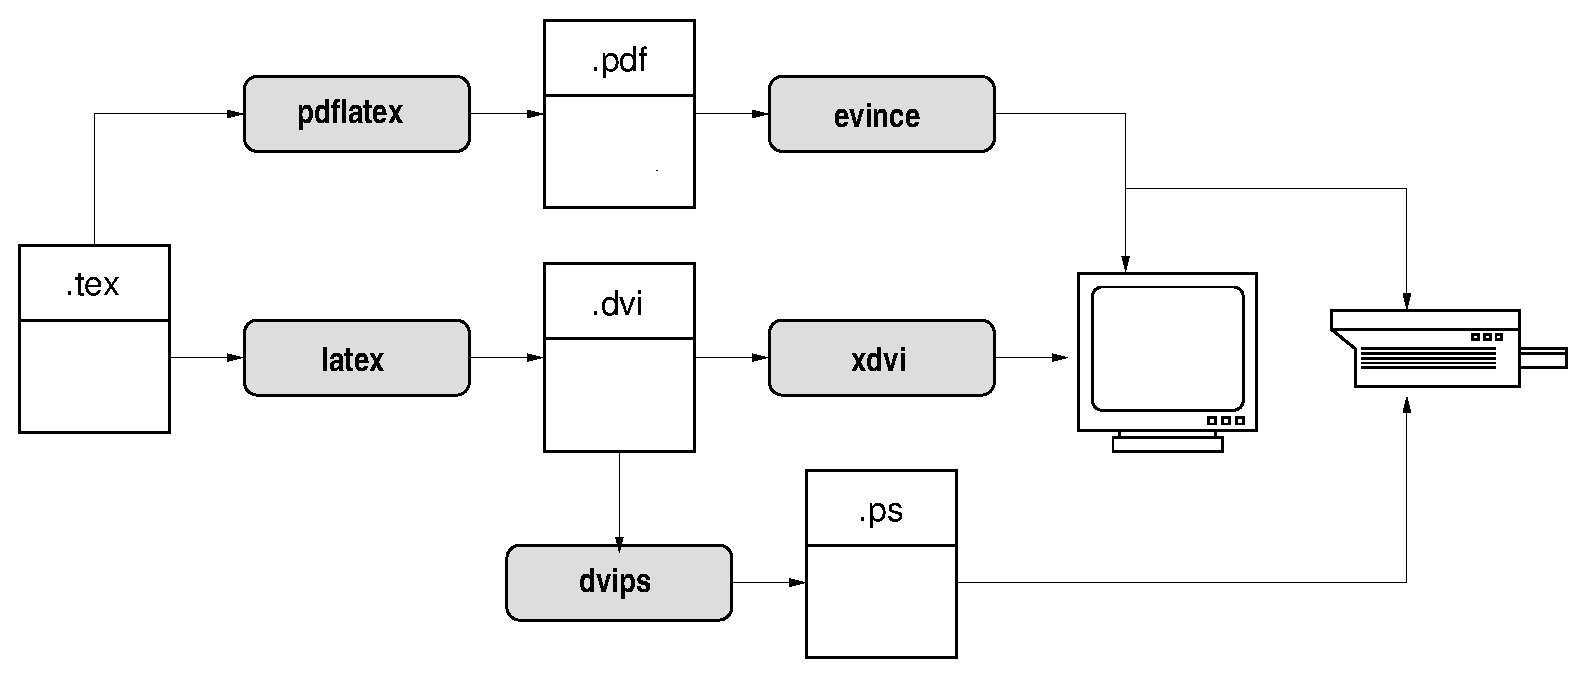
\includegraphics[width = 0.8\linewidth]{img/cycle.eps}
    \caption{UNIX中参与生成过程的工具}
    \label{fig:1.2}
\end{figure}

\subsection{显示}%visualisation有时翻译成可视化,有时翻译成显示,这个可以后期再统一一下。

在编译后,可以简单地使用\textsf{evince}程序来完成显示步骤。输入以下指令:

\dmh{evince \codereplace{文件名}.pdf \&}

这是一个\textsf{linux}下运行的十分直观的程序,能够给出一个方便阅读的文件预览。

\begin{exclamation}
    注意,不必在每次编译后都重新运行evince,它显示的内容会自动刷新。
\end{exclamation}

\subsection{打印}

对于\dm{pdf}格式,如何打印它这一问题就丢给了你的操作系统。关于这一点,没有特殊的注意事项。你有了一个文件,可以自由地处置它,无论是直接打印,还是根据你所处的环境来发挥才艺。

\begin{ii}
    从\dm{dvi}到\dm{ps}格式的转换需要调用dvips程序:

    \dmh{dvips \codereplace{文件名}.dvi}

    这可以生成一个PostScrpt格式的文件。这个格式也由Adobe创造,是一种打印机语言,可以看作\dm{pdf}的祖先。目前的打印机出厂即可识别这种打印机语言。我们可以说,文件发送到打印机时,十有八九传送的是PostScrpt格式的参数。对于PostScript格式的文件,有大量可以显示、修改这种文件的工具。
\end{ii}

\section{源文件的结构}

本节将介绍一种文档类型。实际上,所有\LaTeX 文档都具有相同的结构,形式如下:

\begin{dmd}
\backslash documentclass[\codereplace{类选项$_1$},\codereplace{类选项$_2$},...]\{\codereplace{类}\}\\
\backslash usepackage[\codereplace{包选项$_1$},\codereplace{包选项$_2$},...]\{\codereplace{包}\}\\
...\\
\codereplace{文前部分}\\
...\\
\backslash begin\{document\}\\
...\\
\codereplace{文本}\\
...\\
\backslash end\{document\}
\end{dmd}

如此一来,所有的\LaTeX 文档都可以按以下方式拆解。

\begin{itemize}
    \item 说明文档的\codereplace{类};
    \item 文前部分,包含以下内容:
        \begin{itemize}
            \item 使用特定的\codereplace{包};
            \item 多样的初始化和声明;
        \end{itemize}
    \item 文档主体,即我们将要亲手输入的全部内容,出现在\dm{\backslash begin\{document\}}和\dm{\backslash end\{document\}}之间。
\end{itemize}

以下介绍各部分的细节。

\subsection{文档的类}

所谓类,就是提供给\LaTeX 的一个指示,可以帮助\LaTeX 决定如何为文档的特定部分排版。根据具体使用的类不同,允许使用与否的指令可能不同(如\dm{\backslash chapter}在\dm{book}类中允许使用,在\dm{article}类中不允许使用)。另一方面,根据所选择的类,给出的命令会具有特定的含义(标题、材料表……)。在入门时\jz{
    实际上,我们可以在\dm{\backslash documentclass}前添加更多神奇的“咒语”……
},所有的\LaTeX 文档都必须以的指令开始——\dm{\backslash documentclass}接由花括号括住的类,包含以下几种:

\begin{itemize}
    \item \dm{article},用于文章;
    \item \dm{proc},用于电气与电子工程师协会(英:Institute of Electrical and Electronics Engineers,IEEE)会刊(英:proceeding)风格的文章;
    \item \dm{report},用于几十页篇幅的报告;
    \item \dm{book},用于图书或论文;
    \item \dm{letter},用于信件;
    \item \dm{slides},用于演示文档。
\end{itemize}

我们当然也可以为文档定义自己的类。类的配置项用方括号括住,可以是以下内容之一:

\begin{itemize}
    \item \dm{11pt, 12pt},用于全局地更改文字字号;
    \item \dm{twoside},用于生成适合双面打印的文档;
    \item \dm{draft},用于以草稿模式生成文档。
\end{itemize}

例如,输入:

\begin{dmd}
\verb|\documentclass{article}|
\end{dmd}

以上命令可以将全部配置项配置为默认值(字号为10 pt,单列,单面……)。

\begin{dmd}
    \backslash documentclass[12pt]\{article\}
\end{dmd}

以上命令将字号设置为12 pt(默认为10 pt)。再如:

\begin{dmd}
    \backslash documentclass[twoside, draft]\{report\}
\end{dmd}

以上命令可以以草稿模式生成适合双面打印的报告。

\subsection{文前部分}

文前部分是指位于子句\dm{\backslash documentclass}和子句\dm{\backslash begin\{documennt\}}间的区域。在这个区域中,我们可以明确想要包含的扩展(请看下一小节)%TODO
、初始化全局参数(如页边距等)、定义风格(如标题样式、序号等)、定义特殊的宏,等等。

\subsection{添加扩展}

\LaTeX 命令\dm{\backslash usepackage}可以与C语言的指令\dm{\#include}类比。这一命令允许添加\LaTeX 中满足宏或环境形式的功能\jz{
    相关内容将在下一章讲解。%TODO
}。目前,只需记住,我们可以在一行之内包含多个包:

\begin{dmd}
    \backslash usepackage\{\codereplace{包$_1$},\codereplace{包$_2$},\codereplace{包$_3$},...\}
\end{dmd}

如果\codereplace{包$_1$}、\codereplace{包$_2$}、\codereplace{包$_3$}拥有共同的配置项\codereplace{opt1},我们可以输入:

\begin{dmd}
    \backslash usepackage[\codereplace{opt1}]\{\codereplace{包$_1$},\codereplace{包$_2$},\codereplace{包$_3$}\}
\end{dmd}

相反,如果\codereplace{opt1}只涉及\codereplace{包$_2$},那么我们只能像这样写成两行:

\begin{dmd}
    \backslash usepackage\{\codereplace{包$_1$},\codereplace{包$_3$}\}\\
    \backslash usepackage[\codereplace{opt1}]\{\codereplace{包$_2$}\}
\end{dmd}

下面是两个例子:

\begin{dmd}
    \% 包graphicx带有配置项draft和xdvi\\
    \backslash usepackage[xdvi, draft]\{graphicx\}\\
    \% 包array和包subfig\\
    \backslash usepackage\{array, subfig\}
\end{dmd}

\begin{exclamation}
    根据定义,所有(类、包、命令的)的配置项参数都是\textit{可选的}。因此我们可以这样记:\LaTeX 中所有由方括号括住的参数\dm{[...]}都是非强制的。
\end{exclamation}

\section{开始!}

在本节,我们将尝试从一个只含几个排版命令的文档开始,介绍\LaTeX 的基本原理。

\begin{codelist}[1.1]{
    从你手中掉落的工具总是掉到最难够到的地方,或脆弱的物品上。\\
    这是\emph{墨菲}定律(loi de Murphy)的一个体现。
}  \begin{dmd}
    \verb+\documentclass{article}+\\
    \verb+\begin{document}+\\
    从你手中掉落的工具\\
    总是掉到最难够到的地方,\\
    或脆弱的物品上。\\
    ~\\
    \verb+这是\emph{墨菲}定律(loi de      Murphy)的+\\
    一个体现。\\
    \verb+\end{document}+
\end{dmd}
\end{codelist}

这个示例体现了\LaTeX 中的几个重要的原理,具体如下。

\paragraph*{空行代表跳转至下一段} \LaTeX 中的空行代表一段文字的结尾,因此在以上实例中,第一段从“\dm{从你}”开始,直到“\dm{物品上。}”结束。指令\dm{\backslash par}与空行等价,可以用来表示一段文字的起始。

\paragraph*{\LaTeX 会忽略换行}最终的文档中,换行并不由源文件中的换行决定。\LaTeX 会自动为各段文本\textit{打断、压缩、调节}文字,除非你有特殊的要求。

\paragraph*{\LaTeX 会忽略重复的空格}输入1个或18784个空格是等价的,比如源码中\dm{de}和\dm{Murphy}前插入的空格那样。此规则也适用于跳转段落:输入一行或多行空格是等价的。

\paragraph*{“\backslash ”是转义字符(caractère d’échappement;英:escape char)}“\backslash ”可以告诉\LaTeX 它后面的一系列字符是控制序列,也就是说,是最一般意义上的指令(或宏)。这里,它对“墨菲”一词生效,具体的效果由指令\dm{\backslash emph}控制。

\paragraph*{“\{”和“\}”}它们是\textit{组}的定界符,稍后会进一步解释它们。

\subsection{几个特殊字符}

就像符号“\backslash”的出现所暗示的那样,\LaTeX 中还有10个有特殊含义的符号,在此将其列出:

\begin{dmd}
    \verb+\ $ & % # ^ _ { } ~+
\end{dmd}

%todo 此前代码可以重新简化为verb

以下是一个使用部分特殊字符的案例:

\begin{codelist}[1.2]{
\textbf{是}下标:$x_{i+1}$,还是上标:$e^{i\pi}$;这是问题~1!
}\begin{verbatim}%毫无意义的段落
\textbf{是}下标:$x_{i+1}$,
还是上标:$e^{i\pi}$;
这是问题~1!%还是问题2?\end{verbatim}
\end{codelist}

目前,你需要知道:

\begin{itemize}
    \item \dm{\%}会使得\LaTeX 忽略当前行的剩余部分,因此,它是表示注释的符号(与C中的\dm{//}等价);
    \item \verb+~+代表不可拆分的空格\jz{
        见2.10节。
    },可以防止\LaTeX 在指定的位置断字。尽管有大量的情况需要插入这个符号来表示不可拆分(如所有形如“\verb+图~1+”的情况),然而,对于此类符号的使用,并没有系统化的规则。
    \item \dm{\$}用于标记公式的开始和结束。\LaTeX 遇到一个\dm{\$}符号时,它会切换到\celan{第3章}数学模式,直到遇到下一个\dm{\$}符号。
    \item \dm{\_}和\dm{\^{}}分别代表将文本转化为下标和上标。\textbf{注意},这两个符号只能在数学模式下使用。
    \item \dm{\{}和\dm{\}}分别表示组的开始和结束。本例中出现了两种组:一种出现在数学模式中,用于把将要放到下标或上标的“子公式”组合起来;另一种把将要设置成粗体的文字组合起来。
\end{itemize}

我们可以使用如下的指令来在让文档生成部分特殊字符:

\begin{dmd}
    \verb+\$ \& \% \# \{ \} \_+
\end{dmd}

这串指令可以输出“\$ \& \% \# \{ \} \_”。2.2.5小节%TODO
会解释如何使文档生成其余特殊字符(即\verb+\ ~ ^+)。

\subsection{调用指令}

你已经知道了,要想调用指令或宏,需要输入转义字符,并紧接着输入你想使用的宏名。%TODO 二对一
但是,\LaTeX 如何知道宏名的末尾在哪里呢?此处以用于生成\TeX 标识的\dm{\backslash TeX}为例来解释\yz{
    此例涉及对西文行文中空格的处理,不宜翻译。
}。

\begin{codelist}{
    \TeX book is for \TeX hackers.

    \TeX\  has some powerful macros.

    \LaTeX{} is a document preparation system
}\begin{verbatim}\TeX book is for \TeX hackers.

\TeX\  has some powerful macros.

\LaTeX{} is a document preparation system
    \end{verbatim}
\end{codelist}

\begin{exclamation}
    \verb*|\ |(其中\verb*| |代表空格)称作控制空格(espace de contrôle)。这个空格不会被\LaTeX 忽略。因此,指令“\verb*|et\ \ \ hop !|”会生成“et\ \ \ hop !”。实际上,以\dm{\backslash}\codereplace{函数}\dm{\{}\codereplace{参数}\dm{\}}的形式来调用宏是很好的习惯。因此,使用上例中的的第三种方式比第二种方式更佳。这种形式可以避免空格被忽略的情况发生\jz{
        所以他为什么要跟我们说这些?!
    }。因此,我们将使用\verb|the \teX{}book|来生成“the \TeX{}book”,使用“\verb*|\LaTeX{} is a ...|”来生成“\LaTeX{} is a ...”。
\end{exclamation}

\subsection{变音符号}

法国人往往对于使用\LaTeX 这件事忧心忡忡,因为法文中带有变音符号。别怕!你不必像表\ref{tab:1.1}\yz{
    该表与原书不完全相同。
}中展示的那样输入带有变音符号的字符。然而,你需要知道:无论是什么种类的字符,包括大写字母,我们都可以为其添加变音符号。

\begin{table}[H]
    \centering
    \begin{tabular}{|c|c|c|}
        \hline
        变音符号 & 源码 & 效果\\
        \hline
        尖音符 & \verb|\`z| & \`z \\
        钝音符 & \verb|\'z| & \'z \\
        长音符 & \verb|\^z| & \^z \\
        软音符 & \verb|\c{z}| & \c{z}\\
        分音符 & \verb|\"{z}| & \"{z}\\
        \hline
    \end{tabular}
    \caption{输入占7位(bit)的变音符号}
    \label{tab:1.1}
\end{table}

注意!虽然我们可以输入带有变音符号的字符,但不要忘记:这需要我们调用编码。目前,编码可能只针对地球上的某个地区。在法国,我们使用ISO 8859编码,配合拉丁文1区拓展。这套编码允许我们操纵美丽的变音符号。在详细阅读本书中专为使用法文书写文档的情况准备的章节\celan{第7章}之前,我们建议你在你源码的文前部分添加以下指令,以“攻克”法文文档的难关:

\begin{dmd}
    \begin{verbatim}
%源文件编码
\usepackage[latin1]{inputenc}
%TeX字体编码
\usepackage[T1]{fontenc}
%针对法文文档
\usepackage[francais]{babel}
    \end{verbatim}
\end{dmd}

\section{第一批工具}

以下几个宏和合字在文档中很常用,因此应当了解它们。首先,\LaTeX 会区分三种连接号:

\begin{itemize}
    \item \verb|-|,用于“Saint-Étienne”;
    \item \verb|--|,用于“page 12--24”;
    \item \verb|---|,在法文中用于插入语,如“une parenthèse --- comme cela”。
\end{itemize}

引号应以如下方式输入:

\begin{itemize}
    \item \verb|``|和\verb|''|可以输入英文中的引号\yz{
        此处与原书不同。原书前文输入变音符号时亦直接使用了单弯引号‘和’,但这两个符号作为命令参数时会导致编译错误,因此分别替换为反引号和直单引号。这可能是编译器的差异导致的。
    }——``English''。
    \item 如果键盘允许,对于法文,你可以输入«和»\jz{
        例如,在Linux系统下,分别按键盘的\fbox{Alt Gr}+\fbox{Z}和\fbox{Alt Gr}+\fbox{X}组合键(译注:适用于AZERTY键盘)。
    }。\textsf{babel}包的法文支持部分(参考第7章)%TODO
    允许我们通过\verb|\og|和\verb|fg|输入引号,由此,\verb|\og français\fg{}|这类命令是允许的—— «~français~»~。
\end{itemize}

以下是其余几个使用的命令:

\begin{itemize}
    \item \verb|\today|可以生成(编译时的)日期——2013年11月22日。
    \item \verb|\S|可以生成段落符号——\S。
    \item \verb|\ldots|可以在英文文档中生成省略号“\ldots”。但在法文文档中,应当输入三个点“...”(第7章会介绍更多有关法文排版的内容)。%TODO
\end{itemize}

最后要记得,英文中的双成分标点(ponctuation double;包括:;!?)前不加空格,但法文相反,它们的前面需要加空格。另外,在法国这个可爱的国家,我们几乎都靠右行驶。

\section{第一组报错}

\begin{ii}
    接下来,我们会看看\LaTeX 编译你的文档时闹的“情绪”。当我们放出编译指令时,我们会直接在终端看到这些输出。为了能让\LaTeX 得到充分使用,我们鼓励你在自己的环境下找到属于你自己的检查\LaTeX “\textsf{日志}”的方法。这些日体可以为你指明错误信息,以及编译过程中出现的其他警告。
\end{ii}

\subsection{症状}

如果你与\LaTeX 打交道,那么早晚有一天,你会看到屏幕上显示出类似这样粗旷的信息:

\begin{dmd}
    \linenumbers
    \begin{verbatim}
This is TeX, Version 3.1415 (C version 6.1)
(erreur.tex
LaTeX2e <1995/12/01>
(/usr/local/lib/texmf/tex/cls/article.cls
Document Class: article 1995/11/30 v1.3p Standard LaTeX document class
(/usr/local/lib/texmf/tex/clo/size10.clo)) (erreur.aux)
! Undefined control sequence.
l.5 paragraphe de ce \empha
                           {document}
?\end{verbatim}
\end{dmd}

几乎可以肯定,你看不懂这团内容。它是使用\LaTeX 处理文件\dm{erreur.tex}后终端上显示的内容。以下是文件全文\yz{
    文件正文意为:\dm{我觉得,在这样短的\backslash empha\{文档\}的第一段就有一个错误}。
}:

\begin{dmd}
    \begin{verbatim}
\documentclass{article}

\begin{document}
Il me semble bien qu’il y ait une erreur dans le
premier paragraphe de ce \empha{document} somme
toute assez court.
\end{document}
    \end{verbatim}
\end{dmd}

\subsection{诊断}

我们可以以一种简单的方式来解释以上错误信息。

\paragraph*{第1行}你使用的\TeX 版本为$\pi\pm 10^{-4}$。
\paragraph*{第2行}你想编译文件\dm{erreur.tex}。
\paragraph*{第3行}你使用了\LaTeXe ,版本日期为1995年12月。
\paragraph*{第4行~第5行}你使用了标准文档类\dm{article}。
\paragraph*{第6行}字号默认设置为10 pt。
\paragraph*{第7行}错误信息本身。
\paragraph*{第8行~第9行}\dm{erreur.tex}中造成错误的代码行和对应行号。
\paragraph*{第10行}\TeX 给出的短促且尤其让人焦虑的消息:\dm{?}。

第8行和第9行之间的“裂缝”精准地表明了\LaTeX 崩不住了的地方。以下消息:

\begin{dmd}
    ! Undefined control sequence.
\end{dmd}

向你说明了,\LaTeX 不认识你输入的指令。实际上,指令\verb|\empha|不存在。

\subsection*{治疗方案}

那么,当\LaTeX 给我们展示这个著名的“\dm{?}”时,我们应该怎么回答它呢?这里有3种最简短的方式,可以用来与\LaTeX 轻度交流。

\begin{itemize}
    \item 按回车键来忽略错误。
    \item 输入\dm{x}来退出编译。
    \item 输入\dm{r}让\LaTeX 继续编译,并忽略其他错误信息。
    \item 输入\dm{i}以插入一条更正信息并继续编译,但新插入的更正信息并不会出现在源文档中。
    \item 输入\dm{h}以获取更多关于该错误的信息。以下是本例中\TeX 提供给你的更多信息:\begin{verbatim}
Undefined control sequence :
  The control sequence at the end of the top line
  of your error message was never \def’ed. If you have
  misspelled it (e.g., ‘\hobx’), type ‘I’ and the
  correct spelling (e.g., ‘I\hbox’). Otherwise just
  continue, and I’ll forget about whatever was
  undefined.\end{verbatim}
\end{itemize}

\subsection{一些消息}

\TeX 和\LaTeX 会根据不同的情况给出大量错误消息,其中有一些在第一次面对时并不能读懂。然而,大多数经常出现的消息有以下类型:

\begin{itemize}
    \item \LaTeX 语法或保留字错误;
    \item 花括号没有成对出现;
    \item 在文本模式中出现了本应出现在数学模式中的内容;
    \item 数学模式没有关闭;
    \item 你忘记包含一个包;
    \item 编译过程无法结束;%TODO核实
    \item ……
\end{itemize}

\section{再说几句!}

现在,你知道了如何用\LaTeX 源码创建可打印的文件。同时,本章向你介绍了调用指令的原则。接下来,如果想要了解\LaTeX 语法中的不同功能,需要做的仅仅是去着手接下来的章节。%TODO
% \chapter{(占位)}
\chapter{需要了解的知识}

\begin{epigraphe}{《圣经·箴言》21:11}
    亵慢的人受刑罚,愚蒙的人就得智慧。\\智慧人受训诲,便得知识。
\end{epigraphe}


本章要研究使用\LaTeX 生成文档时的基本排版指令。我们将零散地处理用于突出显示、\LaTeX 标准环境、标题、页面下方的注释、页眉和页脚,以及浮动的环境。接下来,我们会介绍参考系统和\LaTeX 生成的辅助文件。最后,阅读到本章末尾的人将有机会读到一些关于断字的思考。

所有这些指令都将以其默认行为模式使用。也就是说,我们这里不介绍重新定义它们的方法。对应地,你将能够以传统的版式来生成文档。若要打出一篇更进阶的文章,你需要了解如何输入数学式(第3章)、一些关于科技文档的知识(第6章),以及包含图像的方法(第5章)。

\section{突出显示}

要了解\LaTeX 选用字体的机制,需要知道:我们通常通过4个参数来区别字体。

\begin{description}
  \item[族(famille)] 指字体的整体形状。默认情况下,\LaTeX 使用三种字体族:罗马体、\textsf{无衬线体}、\texttt{打字机体}。\LaTeX 中,以英文单词\emph{family}来指代字体族。
  \item[风格(style)] 指字体体现出的样式(英文以\emph{shape}指代),分为:\textit{意大利}、\textsl{倾斜}和小型大写字母风格(\textsc{petites capitales})\yz{
    本书翻译时,以楷体对应意大利风格、以仿宋体对应倾斜风格排版,按原文翻译。中文字体的族和风格往往是并列的,很少有交叉叠加的情况,因此在展示叠加效果时酌情保留原文。中文中很少见到类似小型大写字母的突出显示方式。因此,除了特意展示西文的部分外,本书忽略小型大写字母格式,必要时以其他风格取代。
  }。
  \item [字重(graisse)]指字体笔画的粗细(\LaTeX 中以\emph{serie}指代)。默认情况下有两种粗细:中等和\textbf{加粗}。
  \item [字号]字{\large 体}{\Large 的}{\LARGE 大}{\small 小}。
\end{description}


\subsection{族--风格--字重}

有两种不同的宏可以设置族、风格、字重这三个变量:\emph{指令}和\emph{声明}(如表\ref{tab:2.1}所示)。指令以花括号的形式将其参数括住。声明可以打断行文,同时修改三个变量之一,直到新的命令出现。总体上的规则是,我们使用指令来突出显示一个词或一组词:

\begin{table}
    \centering
    \begin{tabular}{|c|l|c|}
\hline
指令 & 声明 & 输出\\
\hline
\verb+\textrm{...}+ & \verb+{\rmfamily ...}+ & 罗马(roman) \\
\verb+\textsf{...}+ & \verb+{\sffamily ...}+ & \textsf{非衬线(sans sérif)} \\
\verb+\texttt{...}+ & \verb+{\ttfamily ...}+ & \texttt{打字机(machine à écrire)} \\
\hline
\verb+\textup{...}+ & \verb+{\upshape ...}+ & 正(droit) \\
\verb+\textit{...}+ & \verb+{\itshape ...}+ & \textit{意大利(italique)} \\
\verb+\textsl{...}+ & \verb+{\slshape ...}+ & \textsl{倾斜(penché)} \\
\verb+\textsc{...}+ & \verb+{\scshape ...}+ & 小型大写(\textsc{Petites Capitales}) \\
\hline
\verb+\textmd{...}+ & \verb+{\mdseries ...}+ & 中等(médium) \\
\verb+\textbf{...}+ & \verb+{\bfseries ...}+ & \textbf{加粗(gras)} \\
\hline
    \end{tabular}
    \caption{更改字体的声明}
    \label{tab:2.1}
\end{table}

\begin{codelist}[2.1]{
    \texttt{char}类型的\emph{变量}\textsl{总是}被编码为\textbf{8 位}。
}
\begin{verbatim}
\texttt{char}类型的\emph{变量}\textsl{总是}
被编码为\textbf{8 位}。\end{verbatim}
\end{codelist}

注意,在上面的命令中,指令\verb|\emph|(对应的声明是\verb|\em|,可以以更优雅的方式突出显示一组词)。相较声明,强烈建议使用\emph{指令}。当要修改文本的一部分时,使用指令是更明智的选择\jz{定义指令也是。}:

\begin{codelist}[2.2]{
    {\em \bfseries 马格马(Magma) \mdseries 的音乐就像一面镜子,每个人都能看到他自己的倒影。}
}
\begin{verbatim}
{\em \bfseries 马格马(Magma) \mdseries 的音乐
就像一面镜子,每个人都能看到他自己的倒影。}\end{verbatim}
\end{codelist}

接下来的例子展示了如何使用组。声明\verb|\slshape|出现在一个组中,因此它只在组内发挥作用。此外,组会继承它外层的组的参数。这样一来,“silence”一词会使用\textsf{非衬线}体(根据外层的组),并且\textsl{倾斜}展示(根据内层的声明):

\begin{codelist}[2.3]{
    \sffamily 在爵士乐中,{\slshape 沉默(silence)\/}永远是正确的。因此,这是一种充满万千可能的音乐。
}
\begin{verbatim}\sffamily 在爵士乐中,
{\slshape 沉默(silence)\/}永远是正确的。因此,
这是一种充满万千可能的音乐。\end{verbatim}
\end{codelist}

\subsection{意大利体校正}

另一个推荐使用指令而不是声明的理由是,与声明不同,指令可以实现\emph{意大利体校正}。所谓意大利体校正,是指在以意大利体显示的字符组后,有必要增加一个间距,使得这组字符不会“碰到”后面的词。这个间距与所涉及的字符有关\yz{此例展示不同情况下\emph{f}和a间距的细微差距,宜保留原文。例句意为:首长永远是对的。}:

\begin{codelist}[2.4]{
    le {\em chef} a toujours raison.\par
    le {\em chef\/} a toujours raison.\par
    le \emph{chef} a toujours raison.\par
}
\begin{verbatim}
le {\em chef} a toujours raison.\par
le {\em chef\/} a toujours raison.\par
le \emph{chef} a toujours raison.\par\end{verbatim}
\end{codelist}

我们可以看到,指令\verb|\emph|实现了校正,然而,若要使用声明,则需要明确地借助宏\verb|\/|来实现相同的效果。

\subsection{字号}

表\ref{tab:2.2}中展示的宏可以修改行文的字号。这些宏都是\emph{声明}。同时,对于每一个宏都存在同名的环境。

\begin{table}[ht]
    \centering
    \begin{tabular}{|c|c||l|c|}
\hline
\verb|\Huge| & {\Huge 宏大} & \verb|\normalsize| & {正常} \\
\verb|\huge| & {\huge 庞大} & \verb|\small| & {\small 小} \\
\verb|\LARGE| & {\LARGE 特大} & \verb|\footnotesize| & {\footnotesize 加小} \\
\verb|\Large| & {\Large 加大} & \verb|\scriptsize| & {\scriptsize 特小} \\
\verb|\large| & {\large 大} & \verb|\tiny| & {\tiny 微小} \\
\hline
    \end{tabular}
    \caption{修改字号}
    \label{tab:2.2}
\end{table}

\subsection{几个建议}

习惯上,我们应当尽量减少字体变化。实际上,如果字体变化得不合适宜或没有实际用处,尤其是喧宾夺主,影响了文档的可读性,看起来就会很低级。这里是有关使用字体变化的几条建议(仍然是习惯上的建议!):
\begin{itemize}
    \item 相较于使用其余指令,更多地使用\verb+\emph+(默认会将字体改为\emph{意大利}体)。
    \item 将\textbf{加粗}的机会留给特别重要的提示。
    \item 在法文文档中,几乎只在人名中使用小型大写字母(如Donald \textsc{Knuth})。
    \item \dm{打字机}字体族经常被用于生成编程语言的代码或类似的内容。
\end{itemize}

以下内容适用于能读懂其中道理的人……

除以上内容外,我们给出以下两个用于突出显示的情况,读者可以字形斟酌:改变字号、添加下划线(使用指令\verb|\underline|)。

\begin{origincitation}[克努特,\TeX Book{[9]}]
    也许那些希望{\tiny 小声说话}的诗人会让图书的字体频繁变化,但目前,只有一些字体狂人{\tiny (比如本手册的作者)}才喜欢这样做。
\end{origincitation}

\begin{origincitation}[迈克尔·古森斯(Michel Goossens)等,\\《\LaTeX 伴侣》(\emph{\LaTeX{} Companion}){[6]}]
    注意,出版行业认为,以添加下划线的形式来强调内容是不好的习惯。下划线只应用于一种情况——输出设备无法以其他方式突出显示内容,比如使用打字机。
\end{origincitation}

\section{环境}

\LaTeX 以\emph{环境}格式提供了一系列工具,具体结构是一个代码块,语法如下:

\begin{dmd}
    \verb+\begin+\codereplace{环境名}\verb|}|\\
    \verb|...|\\
    \verb+\end+\codereplace{环境名}\verb|}|\\
\end{dmd}

其中\codereplace{环境名}需要替换为具体的环境名称。我们目前遇到的第一个环境是\dm{document}。\verb|\begin| 和\verb|end|间的文字会以特殊版式展示。

\begin{exclamation}
    我们立刻注意到,环境中所有声明都是局部的。另外,当然可以在我们自己定义的环境中套用已经存在的环境。
\end{exclamation}

\subsection{居中和对齐}

想要居中显示几行文字,我们使用环境\dm{center}:

\begin{codelist}[2.5]{
    ……上一段的结尾。
    \begin{center}
        完美居中的\\
        几行文字\\
        且前后带有间距
    \end{center}
    然后继续下一段……
}
\begin{verbatim}
……上一段的结尾。
\begin{center}
  完美居中的\\
  几行文字\\
  且前后带有间距
\end{center}
然后继续下一段……\end{verbatim}
\end{codelist}

同样,我们可以轻易地借助环境\dm{flushright},让一个段落右对齐排列:

\begin{codelist}[2.6]{
    ……上一段的结尾。
    \begin{flushright}
      两行右对齐\\
      的文字
    \end{flushright}
    然后继续下一段……
    }
\begin{verbatim}
……上一段的结尾。
\begin{flushright}
  两行右对齐\\
  的文字
\end{flushright}
然后继续下一段……\end{verbatim}
\end{codelist}

注意,以上两个示例中,命令\verb|\\|起到了换行的功能。除一些特殊场景(表格、文档的标题和作者、特意的居中或对齐处理)外,不要使用这个命令——如果想要换行,需要使用空行或命令\verb|\par|。

\begin{flushleft}
    一般情况下,我们使用环境\dm{flushleft}时需要搭配命令\verb|\\|。但我们可以使用这个环境来生成右侧不对齐的文档,将换行的麻烦工作留给\LaTeX ,就像这段文字一样。(\textsl{译注}:此处给出本段原文。请注意右侧的换行的不对齐处理。En général, on emploie l'environnement \dm{flushleft} avec des commandes \verb|\\|. Mais on peut l'utiliser pour produire un paragraphe comme celui-ci, non justifié à droite, en laissant à \LaTeX{} le soin d’insérer les sauts de lignes.)
\end{flushleft}

%TODO 排查代码下正文内容
\begin{exclamation}
    绝大部分环境都会重启一行来插入内容。然而,重要的是:环境只是在插入内容的位置\emph{中断}当前段落,而不是结束当前段落。你可以在前两个实例中看到,“然后继续下一段……”这句话前没有缩进。另外,\LaTeX 贴心地在每个环境前后都留了一段空白。
\end{exclamation}

我们可以注意到,前面的三个环境分别代表以下三个声明:

\begin{itemize}
    \item \verb|\centering|;
    \item \verb|\raggedleft|;
    \item \verb|\raggedright|。
\end{itemize}

例如,我们可以这样写\yz{
    实际上,Emacs代表Editor MACroS。本例是对Emacs的调侃。
}:

\begin{codelist}[2.7]{
    Emacs代表:

    {\centering Emacs\\Makes\\
      A\\Computer\\Slow\\}
}
\begin{verbatim}
Emacs代表:

{\centering Emacs\\Makes\\
  A\\Computer\\Slow\\}\end{verbatim}
\end{codelist}

\subsection{列表}

\LaTeX 提供了三种呈现\emph{列表}的基本环境:\dm{itemize}、\dm{enumerate}、\dm{description}。如果它们都不能满足你,也可以定义属于你自己的\celan{9.5节}列表。但目前,先来看看标准的列表。

首先,\dm{itemize}可以生成不编号的项目列表。在法文版本中,一级列表会使用连接号(---)标记;在其他版本中,会使用点($\bullet$)标记:

\begin{codelist}[2.8]{
……一句话的结尾。
\begin{itemize}
\item 在复杂的计算中,分子的系数需要传递给分母;
\item 不应当写逗号。
\end{itemize}
然后行文继续。
}
\begin{verbatim}
……一句话的结尾。
\begin{itemize}
\item 在复杂的计算中,
  分子的系数需要
  传递给分母;
\item 不应当写逗号。
\end{itemize}
然后行文继续。\end{verbatim}
\end{codelist}

环境\dm{enumerate}遵循类似的规则,只不过项目会被编号。一个环境中可以套用另一个环境。下面的例子中,我们同时展示了\dm{ enumerate}和\dm{description}环境:

\begin{codelist}[2.9]{
    ……还是一句话的结尾。
    \begin{description}
    \item[\TeX] \TeX{}book;
    \item[\LaTeX] 两本重要的书:
      \begin{enumerate}
      \item 《\LaTeX{}:一个文档准备系统》(\emph{\LaTeX{}: A Document Preparation System})。
      \item 《\LaTeX{}伴侣》。
      \end{enumerate}
    \end{description}
    跟之前一样,接下来段落继续……
}
\begin{verbatim}
……还是一句话的结尾。
\begin{description}
\item[\TeX] \TeX{}book;
\item[\LaTeX] 两本重要的书:
  \begin{enumerate}
  \item 《\LaTeX{}:一个文档
    准备系统》(\emph{\LaTeX{}: 
    A Document Preparation System})。
  \item 《\LaTeX{}伴侣》。
  \end{enumerate}
\end{description}
跟之前一样,接下来段落继续……\end{verbatim}
\end{codelist}

至于环境\dm{description}的列表,在我们习惯的文档处理中没有对应内容。不幸的是,对于\LaTeX 初学者,它最好的结果是被误用,最差的结果是被无视。

\subsection{制表}

环境\dm{tabbing}可以用于打字机上使用的那种老式制表过程%TODO查证
。我们可以使用指令\verb|\=|来放置定位标记,并使用指令\verb|\>|来在定位标记之间移动。此外,\verb|\\|可以用来换行。

\begin{codelist}[2.10]{
  \begin{tabbing}
    左倾 \= 中间立场 \= 右倾 \\
    \> 中立派 \\
    \> \> 保守派 \\
    xxxxxxxxx \= \kill
    \> 无观点
    \end{tabbing}
}
\begin{verbatim}
\begin{tabbing}
  左倾 \= 中间立场 \= 右倾 \\
  \> 中立派 \\
  \> \> 保守派 \\
  字字字字字 \= \kill
  \> 无观点
\end{tabbing}\end{verbatim}
\end{codelist}

我们可以从这个例子中看到两个规则:

\begin{itemize}
    \item 可以在制表时插入一行“模板”,并且使用指令\verb|\kill|来隐藏这一行;
    \item 如果已经存在定位标记,新的指令\verb|\=|可以在逻辑上移除它们。
\end{itemize}

\subsection{表格}

\LaTeX 中用于生成\emph{表格}的环境称为\dm{tabular}。表线的处理可能不太精细,但对于线条简单的表格,结果可以接受\jz{
    附录B提供了一些提示,可以用来找到能够生成更复杂表格的包。
}:

\begin{codelist}[2.11]{
    嚯:
    \begin{tabular}{|r|c|}
        \hline
        俩 & 仨 \\
        五个 & 六个  \\ \hline
      \end{tabular}
}
\begin{verbatim}
嚯:
\begin{tabular}{|r|c|}
  \hline
  俩 & 仨 \\
  五个 & 六个  \\ \hline
\end{tabular}\end{verbatim}
\end{codelist}

通过这个例子,我们可以得到以下结论。

\begin{itemize}
    \item 环境\dm{tabular}会等待输入一个参数,应用指示表格的格式。每列都应该以一个定位字符表示。
    \begin{itemize}
        \item \dm{r}:右对齐。
        \item \dm{c}:居中。
        \item \dm{l}:左对齐。
    \end{itemize}
    \item 字符\verb|&|用于分隔不同列。
    \item 指令\verb|\\|用于跳转至下一行。
    \item 布局字符串中的\dm{|}表示插入纵向表线。
    \item 横向表线由指令\verb|\hline|插入。
\end{itemize}

因此,我们可以自由地调整\verb|\hline|和\dm{|}的数量,以隐藏或显示表线。包\textsf{array}可以满足一些关于表格的幻想。

\begin{exclamation}
大多数环境都会另起一行,但\dm{tabular}不会。\dm{tabular}会紧接当前的文本生成\linebreak 表格。
\end{exclamation}

此外,我们还可以使用参数来精确地指定表格竖直方向上的位置:

\begin{codelist}[2.12]{
一个表:\begin{tabular}[b]{|c|} 
甲\\乙
\end{tabular}
,另一个表:\begin{tabular}[t]{|c|} 
丙\\丁\end{tabular}
}
\begin{verbatim}
一个表:\begin{tabular}[b]{|c|} 
  甲\\乙
\end{tabular}
,另一个表:\begin{tabular}[t]{|c|} 
  丙\\丁
\end{tabular}\end{verbatim}
\end{codelist}

我们可以看出,参数\dm{b}将表格“放置”在当前行上,参数\dm{t}将表格“悬挂”在当前行下。如果没有参数,表格会在竖直方向上居中,就像前面的例子一样。

显然,表格可以不插入句子中,而可以单独成段,比如配合环境\dm{center}被单独居中。

\subsection{模拟终端}

环境\dm{verbatim}可以将其内容逐字插入文档。因此,无论什么字符,甚至是特殊字符,都可以使用它来插入,如插入一个\textsf{C++}代码片段:

\begin{codelist}[2.13]{\ttfamily
  \begin{tabbing}
    cl\=ass pixel \{\\
      \>int x, y;\\
    public:\\
      \>pixel(int i=0, int j=0);\};
  \end{tabbing}
}
\ttfamily
\backslash begin\{verbatim\}
\begin{verbatim}
class pixel{
  int x,y;
public:
  pixel(int i=0, int j=0);};\end{verbatim}
\backslash end\{verbatim\}
\end{codelist}

\begin{exclamation}
我们可以在环境\dm{verbatim}中写任何内容,\emph{除了}以下字符串——\verb|\end{verbatim}|!\\
\end{exclamation}

有两个指令可以像\dm{verbatim}一样生成文本片段:\verb|\verb|和\verb|\verb*|。带有星号的版本可以将空格“\verb| |”显示为“\verb*| |”的形式。

这两个指令的参数不使用花括号括起,而夹在任何一种可以满足以下两个条件的符号之间:不能是特殊符号、不能在参数中包含:

\begin{codelist}[2.14]{
  使用{\ttfamily \#include<stdlib.h>}可以
  包含C语言标准库的原型。
}
\begin{verbatim}
使用\verb+#include<stdlib.h>+可以
包含C语言标准库的原型。\end{verbatim}
\end{codelist}

\begin{exclamation}
在任何情况下,指令\verb|\verb|都不能出现在其他指令的参数中,无论这个指令是\linebreak 什么。
\end{exclamation}

\subsection{引用语}

环境\dm{quote}和\dm{quotation}可以在文本中引用内容。首先来看\dm{quote}:

\begin{codelist}[2.15]{
  ……仍然是一句话的结尾。
\begin{quote}
  万物相关。\hfill\textbf{爱因斯坦}

  有件事情是不确定的,
  那就是所有事情都是确定的。
  \hfill\textbf{帕斯卡}
\end{quote}
然后继续被打断的段落……
}
\begin{verbatim}
……仍然是一句话的结尾。
\begin{quote}
  万物相关。\hfill\textbf{爱因斯坦}

  有件事情是不确定的,
  那就是所有事情都是确定的。
  \hfill\textbf{帕斯卡}
\end{quote}
然后继续被打断的段落……\end{verbatim}
\end{codelist}

指令\verb|\hfill|可以插入一段在水平空间上\celan{\S 4.2.4}无限延伸的空白。环境\dm{quotation}有一些细微的差别:

\begin{codelist}[2.16]{
  ……仍然是一句话的结尾。
\begin{quotation}
  人有许多缺陷,但我们若能
  想到他们被创造的那个年代,
  就能对此感到宽容。\par
  \raggedleft 阿方斯·阿莱
  (Alphonse Allais)
\end{quotation}
然后继续被打断的段落……
}
\begin{verbatim}
……仍然是一句话的结尾。
\begin{quotation}
  人有许多缺陷,但我们若能
  想到他们被创造的那个年代,
  就能对此感到宽容。\par
  \raggedleft 阿方斯·阿莱
  (Alphonse Allais)
\end{quotation}
然后继续被打断的段落……\end{verbatim}
\end{codelist}

实际上,对于这两个环境,根据莱斯利·兰波特的介绍,一个(\dm{quote})是为引用一条或多条短的内容而准备的,另一个(\dm{quotation})是为引用一条长的内容而准备。

\section{页边注}

指令\verb|\marginpar|可以在页边缘创建一个小段落,语法如下:

\begin{dmd}
\backslash marginpar\{\codereplace{文字}\}
\end{dmd}

对于双面打印的模式,为了区分左侧和右侧的页面,我们可以使用如下指令\yz{
  原书有误。此处已更正。
}:

\begin{dmd}
\backslash marginpar[\codereplace{左侧文字}]\{\codereplace{右侧文字}\}
\end{dmd}

其中\codereplace{左侧文字}和\codereplace{右侧文字}会根据当前页码的奇偶性在页面左侧或右侧呈现。如此一来,以下指令:

\begin{dmd}
\backslash marginpar[这!]\{嚯!\}
\end{dmd}\marginpar[这!]{嚯!}

会生成你在本页页边缘看到的内容。

\section{标题}

表\ref{tab:2.3}给出了\LaTeX 种可用的\emph{章节}命令。对于类型为\dm{article}的文档,指令\verb|\chapter|不可用;对于类型为\dm{letter}的文档,任何标题类型都不可用。目前,你需要了解以下两点:

\begin{itemize}
  \item 使用指令生成的每个标题都可以自动\emph{编号},并可以在必要时列入目录。
  \item 使用指令\verb|\tableofcontents|可以生成目录,并将其插入该指令所在的位置。
\end{itemize}

\begin{table}[ht]
  \centering
  \begin{tabular}{|l|l|l|}
    \hline
    \verb|\part{...}| & \verb|\chapter{...}| & \\
    \verb|\section{...}| & \verb|\subsection{...}| & \verb|\subsubsection{...}| \\
    \verb|\paragraph{...}| & \verb|\subparagraph{...}| &  \\
    \hline
  \end{tabular}
  \caption{章节指令}
  \label{tab:2.3}
\end{table}

\begin{ii}
此外,所有的标题指令都带有可以自定义的相关类型。% TODO
总的来说,这些指令会自动生成标题前后的间距。如此一来,指令前后的任何空行都会被忽略。
\end{ii}

\begin{codelist}[2.17]{
  ……一句话的结尾。
  \section*{3.2\quad 结论}
  最终,……
}
\begin{verbatim}
……一句话的结尾。
\section{结论}
最终,……\end{verbatim}
\end{codelist}

每种标题指令都带有一种“带星”形式(例如,\verb|\section*|),可以插入不参与编号的标题。但需要注意,这种标题不会出现在\celan{\S 2.9.2}目录中。与节(section)相关的标题指令中可以接受参数,用于明确目录中展示的内容。例如:

\begin{dmd}
\verb+\section[张三]{太帅了!}+
\end{dmd}

可以在文档中插入节标题“太帅了!”,但在目录中将其展示为“张三”。

\section{页面底部的注释}

有一种方便的方式可以在页面底部插入注释:使用指令\verb|\footnote{|\codereplace{文本}\verb|}|。注释会自动编号,且在默认情况下按章重新编号。如下是\LaTeX 可以实现的效果:

\begin{codelist}[2.18]{
  无论如何,指令\texttt{footnote}$^a$可以在页面底部插入注释。\\
  ————\\%TODO 
  {\footnotesize $^a$正如其名。}
}
\begin{verbatim}
无论如何,指令\verb+footnote+
\footnote{正如其名。}可以在页面
底部插入注释。\end{verbatim}
\end{codelist}

在一些特殊情况中,\verb|\footnote|不能生成我们想要的效果。此时,有必要分两步走:

\begin{enumerate}
  \item 使用指令\verb|\footnotemark|放置\emph{注释标记};
  \item 当条件允许时,使用指令\verb|\footnotetext|在页面底部输入\emph{文字}。
\end{enumerate}

例如,在表格中插入注释似乎有点棘手,此时可以这样写:

\begin{codelist}[2.19]{
  \begin{tabular}{cc}
    甲 & 乙$^a$ \\
    丙 & 丁\\
  \end{tabular}\\
  ————\\
  {\footnotesize $^a$一个注释。}
}
\begin{verbatim}
\begin{tabular}{cc}
  甲 & 乙\footnotemark \\
  丙 & 丁
\end{tabular}\footnotetext{一个注释。}\end{verbatim}
\end{codelist}

\section{页眉和页脚}

\LaTeX 生成页眉和页脚的标准指令有些简陋,但这里也值得一提,因为这些指令对于一些特定情况已经足够了。

\begin{ii}
关于这些指令,在这里就不讲更多内容了,因为\dm{fancyhdr.dvi}中介绍的fancyhdr包易用得多,也提供了比\LaTeX 的标准指令多得多的有趣选项。本书关于使用此包生成页眉页脚的详细解释在10.4节。
\end{ii}

如果不调用其他包,可以在文档的文前部分使用指令\verb|\pagestyle|来指定页眉页脚的风格:

\begin{dmd}
\verb|\pagestyle{|\codereplace{风格}\verb|}|
\end{dmd}

其中,参数\codereplace{风格}可以从以下值中选择:

\begin{itemize}
  \item \dm{empty},不显示页眉和页脚;
  \item \dm{plain},默认风格,页脚居中显示当前页码;
  \item \dm{headings},在页眉显示一定的内容,根据文档风格的不同而不同(例如,在双面的\dm{report}文档中,会显示当前的章名或节名);
  \item \dm{myheadings},自定义插入内容。
\end{itemize}

此外,使用指令\verb|\thispagestyle|,可以变更或指定当前页的风格。

\section{浮动环境}

\LaTeX 为其优秀的用户提供了使用\emph{浮动}环境的可能性。这种环境的特点是,其内容会被“漂浮地”渲染到正文中。也就是说,\LaTeX 通过一种算法,综合考虑一系列参数,在文档中为这种环境挑选位置。

\begin{exclamation}
\LaTeX 中的环境\dm{figure}和\dm{table}并不仅仅可以用来插入图片和表格,这一点与它们的名字相反。实际上,这两种环境只是将其内容浮动起来,并且为添加图题或表题提供了可能性。实际上,这两种环境中可以是你喜欢的任何内容,也不一定要是图形。
\end{exclamation}

\subsection{图(figure)和表(table)}

环境\dm{figure}一般用来插入图像,而环境\dm{tale}一般用于插入表格。这两种环境都可以带有自己的小标题,使用语法如下:

\begin{codelist}[2.20]{
  此段包含了浮动环境“figure”,
其内容可以在页面中浮动。
% \begin{figure} 插环境会报错
  \begin{center}
三\\
O丁O\\
四\\
Figure 1: 有个老丁头
  \end{center}
%   \caption*{有个老丁头}
% \end{figure}

}
\begin{verbatim}
此段包含了浮动环境“figure”,
其内容可以在页面中浮动。
\begin{figure}
  \begin{center}
    三\\
    O丁O\\
    四\\
  \end{center}
  \caption{有个老丁头}
\end{figure}\end{verbatim}
\end{codelist}

注意到,使用指令\verb|\caption|可以生成图题或表题。文本“Figure 1:”会自动生成,并给出对应该图片的编号。这种“风格”也是可以自定义的。

\subsection{确定位置}

我们可以在\verb|\begin|后面用方括号中给出参数,来让\LaTeX 尝试依此放置浮动的内容,具体如下:

\begin{itemize}
  \item \dm{h},放置在源码中出现的原位置;
  \item \dm{t},放置在页面顶部;
  \item \dm{b},放置在页面底部;
  \item \dm{p},放置在单独的页面上。
\end{itemize}

注意,有时我们会为如何放置浮动环境而抓狂。为了不因此而烦躁,需要理解(并接受)下面这一点:\LaTeX 会综合考虑多个参数来安排环境\dm{figure}和\dm{table}的位置,其中包括:

\begin{itemize}
  \item 放置在页面顶部和底部的浮动环境的最大数量;
  \item 顶部和底部放置有浮动环境的页面占全部页面的最大可接受比例;
  \item 浮动环境前后的空白。
\end{itemize}

如果你在放置图片时遇到了关于其位置的问题\jz{并且你确定它真的成问题……},我们建议你遵循以下建议:

\begin{itemize}
  \item 如果你尝试写“\textsl{如下图所示:}”之类的话,并且希望紧接着放一个图片,\emph{不要使用环境}\dm{figure}!。
  \item 尽量使用\emph{参考}系统,例如写成“如图3所示”。
  \item 我们总是喜欢放一些超大图片——缩小它们!
  \item 如果你的表格太长,把它放到附录中去。无论如何,它会让读者很难受。
  \item \LaTeX 中的参数经过精心研究,目的是平衡文档中文字和图片的数量。所以如果你的文档是连环画,请做好最坏的准备……
  \item 只有到了\textbf{印刷你的最终版文档}时才有必要去纠结图片的位置。
\end{itemize}

\subsection{图片列表}

使用指令\verb|\listoffigures|(对应地,\verb|\listoftables|)可以在文档中插入全部图片(对应地,表格)的列表。列表会出现在指令所在的位置。此类指令会生成扩展名为\dm{.lof}(对应地,\dm{.lot})的文件。此外,与插入节标题时使用参数指定目录中展示的内容类似,指令\verb|\caption|中也可以带有一个参数,来控制其在列表中显示的内容。默认情况下,列表中会显示图题(对应地,表题):

\begin{dmd}
\verb|\caption[嚯]{|你可以在这里尽情写些人生故事,因为无论你写多长,它都不会出现在图片列表中,因为我们已经指定了这个无比长的小标题显示成“嚯”……\verb|}|
\end{dmd}

\section{引用}

\LaTeX 的引用系统以为对象编号的方式允许你以符号的方式操作文档中任何部分的序号,因此,没有必要去记忆一个图片究竟是图4还是图5。\LaTeX 通过这种方式为你减少了很多工作,并且这种方式可以通过几行文字就能解释清楚。

\subsection{原理}

为了在文档中成功使用引用,我们需要做两件事:第一,在文档中添加符号标记;第二,调用这个标记来进行引用,要么引用相应对象的序号,要么引用其出现的页码。这样简单的方式简化了工作:

\begin{enumerate}
  \item 使用指令\verb|\label|来添加标记:\\
  \verb|\label{|\codereplace{标记内容}\verb|}|\\
  其中\codereplace{标记内容}是一个不带有特殊字符的字符串;
  \item 使用指令\verb|\ref|来引用相应对象的序号:\\
  \verb|\ref{|\codereplace{标记内容}\verb|}|
\end{enumerate}

使用\verb|\pageref|,可以引用相应页码:

\verb|\pageref{|\codereplace{标记内容}\verb|}|

\subsection{需要引用什么?}

我们可以引用的内容如下:

\begin{itemize}
  \item 各级标题;
  \item 浮动环境(\dm{figure}、\dm{table}……);
  \item 数学式(参见第3章);
  \item 带编号列表(如\dm{enumerate})的项;
  \item 等等。
\end{itemize}

如下的示例综合了三种引用指令:

\begin{codelist}[2.21]{
  \section*{3.5\quad 二次方程}
二次方程即以下形式的方程 :
\begin{equation}
  ax^2 + bx + c = 0 \tag{2.12}
\end{equation}
第13页3.5节中的方程2.12这么说完那么说……
}
\begin{verbatim}
\section{二次方程}\label{sec-2dg}
二次方程具有以下形式 :
\begin{equation}
  ax^2 + bx + c = 0 \label{equ}
\end{equation}
第\pageref{sec-2dg}页\ref{sec-2dg}节
中的方程\ref{equ}这么说完那么说……\end{verbatim}
\end{codelist}

在这个示例中,我们引用了对象\verb|\section|和另一个\verb|\equation|。此外,我们还引用了这个关于方程的节所在页的页码。

\begin{exclamation}
当在浮动环境中放置\verb|\label|时,请一定将其放置指令\verb|\caption|的\textbf{后面}。否则,引用会“指向”当前的节,而不是图形。
\end{exclamation}

\section{辅助文件}

为了进一步理解引用的机制,我们需要检查以下\LaTeX 编译源文件时向你的硬盘中写入了什么。目前,你可以看到的文件有如下格式。

\begin{description}
  \item[\fbox{\texttt{dvi}}] 文档中的图片。
  \item[\fbox{\texttt{log}}] \LaTeX 在最近一次编译时的“自言自语”。一般情况下,它多多少少代表了你编译时在终端上看到的内容。
  \item[\fbox{\texttt{aux}}] 辅助文件,储存引用、页码、标题等信息。
  \item[\fbox{\texttt{toc}}] 目录文件。
  \item[\fbox{\texttt{lof}}] 图片列表文件。
\end{description}

\subsection{与引用的交互}

\LaTeX 以如下的方式处理引用:在第一次编译时,在文件\codereplace{文件名}\dm{.aux}中储存引用,其中\codereplace{文件名}是你的文档的文件名。我们可以在如下示例中看到其解决引用的问题时的机制和原理,在该示例中,我们尝试引用位于第35页的第3节中的一个名为\dm{truc}的标记\yz{“truc”意为“小东西”。}。

\begin{enumerate}
  \item 在第一次编译时,\LaTeX 在\dm{.aux}格式的辅助文件中存储该标记的号码(在本例中,存储其所在节的序号)和该标记出现页的页码(如图\ref{fig:ref1}所示)。
  
  \begin{figure}[ht]
    \begin{center}
      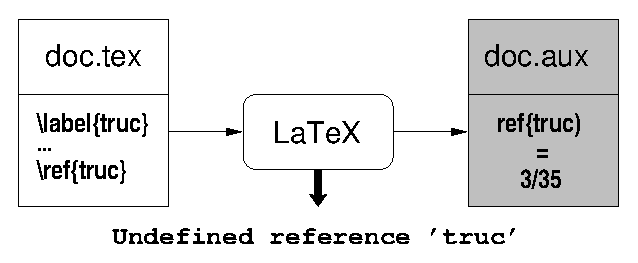
\includegraphics{img/ref1.eps}
    \end{center}
    \caption{使用\dm{.aux}的第一次编译}
    \label{fig:ref1}
  \end{figure}

  因此,此次编译时,会\LaTeX 发送警告,指出标记\dm{truc}未定义。
  \item 我们会进行第二次编译,这次编译会使用辅助文件的内容(如图\ref{fig:ref2}所示)。
  
  \begin{figure}[ht]
    \begin{center}
      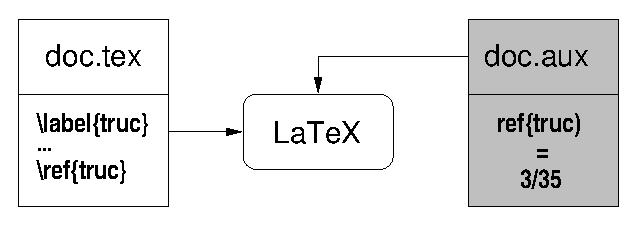
\includegraphics{img/ref2.eps}
    \end{center}
    \caption{使用\dm{.aux}的第二次编译}
    \label{fig:ref2}
  \end{figure}
\end{enumerate}

在以下情况中的引用定义是不正确的。

\begin{enumerate}
  \item 你插入了一个新的标记,并且在插入标记后第一次编译(引用\emph{未被定义})。此时,对于新插入的标记,会得到如下形式的消息:
  
  \begin{dmd}
  Reference 'vlunch' on page 2 undefined on input line 17.
  \end{dmd}

  \item 你在文档中引入的变化无疑会改变页码或对象(图片、方程等)的位置,因此引用会被\emph{错误定义}。在编译结束时,你会看到如下警告:
  
  \begin{dmd}
  Label(s) may have changed.\\
  Rerun to get cross-references right.
  \end{dmd}

  \item 你引用了一个不存在的标记。在这种情况下,再编译八百次也无济于事。
\end{enumerate}

\subsection{与目录的交互}

对于目录,你会发现,其原理与引用是类似的。在文档中插入指令\verb|\tableofcontents|意味着目录将会分两步创建,具体如下。

\begin{enumerate}
  \item 第一轮遍历会收集文档中与\emph{表题}相关的信息,并将其存入文件\codereplace{文件名}\dm{.toc}中(如图\ref{fig:toc1}所示)。
  
  \begin{figure}[ht]
    \begin{center}
      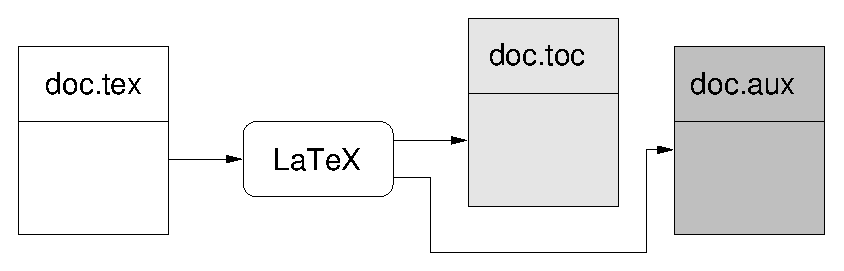
\includegraphics{img/toc1.eps}
    \end{center}
    \caption{使用\dm{.toc}的第一次编译}
    \label{fig:toc1}
  \end{figure}

  \item 第二轮遍历会使最终的文档中包含\codereplace{文件名}\dm{.toc},因此,目录也会被包含(如图\ref{fig:toc2}所示)。
  
  \begin{figure}[ht]
    \begin{center}
      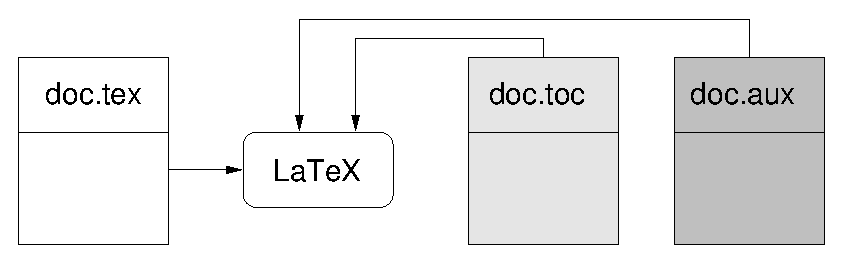
\includegraphics{img/toc2.eps}
    \end{center}
    \caption{使用\dm{.toc}的第二次编译}
    \label{fig:toc2}
  \end{figure}

\end{enumerate}

你可能会遇到这种情况:在写草稿时,文档已经包含了目录指令(\verb|tableofcontents|),而你又添加了新的章节指令。在这种情况下,新的章节只有经过\textbf{两次}编译后才会显示在目录中。

\subsection{一些建议}

要养成为每个文档生成目录的习惯。实际上,\LaTeX 会围绕你的\dm{.tex}文件生成多个文件\jz{
  这还没有涉及参考文献、索引、术语目录等。
}。另外,在起草文档时,不必过于关心目录是否时刻更新——它早晚会更新的!实际上,只有在\textbf{印刷}之前才有必要去确认所有的引用都是正确的。

最后,就像我们在不再能确定目标文件时会时不时运行一下\dm{make clean}指令一样,在看起来一切都运行不正常时,删掉辅助文件\celan{\S B.2}并重新编译是个好习惯。

\section{断字的处理}

\LaTeX 依靠\TeX 对特定的语言来实现不同的断字效果。这种算法在\TeX Book的附录H中有描述,也体现出\TeX 最成功的一面。通过检查文档打断段落的方式,可以识别出文档是不是由\LaTeX 生成的,因为其他很多软件都喜欢以在单词间添加更多空间的方式来处理此类问题。然而,也会有一些\LaTeX 无法正确断字的情况。在这种情况下,\LaTeX 会以以下两种“吓人的”信息之一为你给出警告:

\begin{dmd}
Underfull \backslash hbox (badness 1810) detected at line 33
\end{dmd}

或

\begin{dmd}
Overfull \backslash hbox (14.24376pt too wide) detected at line 41
\end{dmd}

\TeX 在很底层用你的文档生成一系列\emph{字盒}。每个字符都装入合适的字盒,字盒组合成词,再以类似的方式组合成行、成段,然后成页面。

这里以一种简单的方式总结和介绍原理。我们可以简单地理解为,\TeX 在水平模式下操纵\verb|\hbox|来组合单词,在竖直模式下操纵\verb|\vbox|来生成页面。此外,组合这些字盒时,\TeX 如果觉得结果不太美观,就会用以上述两种信息警告你。信息的含义如下。

\begin{itemize}
  \item \verb|Underfull \hbox|表示字盒组合得有些稀疏。通过显示badness的值,\TeX 会告诉你它认为当前行“有多丑”。如果一行文字排列得很完美,该值为0。在最差的情况下,该值为10000.
  \item \verb|Overfull \hbox|表示字盒有些太挤了。\TeX 可以以\dm{pt}为单位显示文字越界深入边缘的长度。
\end{itemize}

如果一个页面过于稀疏,\LaTeX 会以\verb|\vbox|代替\verb|\hbox|显示类似的消息。表\ref{tab:2.4}展示了同一句话的不同疏密程度\yz{
  表中的例句出自法国古典主义戏剧大师高乃依(Pierre Corneille)的戏剧《熙德》(\textit{Le Cid}),意为“哦,愤怒!哦,绝望!哦,宿敌!”。
}排列效果。

\newcommand{\phrase}[1]{\noindent\makebox[\width +
#1][s]{%
  Ô rage ! ô désespoir ! ô vieillesse ennemie !}\par}
\begin{table}[ht] 
\begin{center}
  % \addtolength{\extrarowheight}{4pt} 
  \begin{tabular}{|l|c|}
    \hline
    效果 & 评价 \\
    \hline
    % \typeout{UNDERFULL HBOX AUTORISE}%
    \phrase{1.0cm}  & 稀疏\\
    \phrase{0.75cm} & 稀疏\\
    \phrase{0.45cm} & 稀疏\\
    \hline
    % \typeout{UNDERFULL HBOX AUTORISE}%
    \phrase{0cm}    & 理想 \\ 
    \hline
    \phrase{-0.1cm} & 过密\\
    \phrase{-0.2cm} & 过密\\
    \phrase{-0.25cm} & 过密\\
    \hline
  \end{tabular}
  \caption{横向的不同疏密排列}
  \label{tab:2.4}
\end{center} 
\end{table}

\begin{ii}
  \makebox[\width+2pt][s]{可以在文档选项中启用\dm{draft},来使在出现\dm{Overfull \backslash hbox}问题的位置的侧栏显示一个黑色的\char"258C}
  方块,就像本段的侧栏一样。这个选项可以帮助快速定位导致问题的行。
\end{ii}

\subsection{控制断字}

对于以下情况,\LaTeX 的断字处理可能遇到困难。

\begin{itemize}
  \item 它不能识别需要打断的词——这是个极端情况。
  \item 不能打断的对象占据了需要打断的位置,例如\verb+\verb|...|+或方程类型的对象。
\end{itemize}

这里提供以下几个控制断字的方法。

\begin{exclamation}
如果以下方法都不能使你满意(如果你的句子中包含太多\TeX 不能打断的对象,就会产生这种情况),就只能想办法更换表达方式来规避问题了。
\end{exclamation}

\subsubsection{引导断字}

我们可以通过在必要的位置插入指令\verb|\-|来指出可以断字的位置,从而帮助\LaTeX 实现断字。例如,如果\LaTeX 不能成功地打断“nonmaiçavapamieu”\yz{
  作者的生造词,形似句子“Non, mais ça ne va pas mieux.”,意为“不,没有变得更好”。
}一词,我们可以输入:

\begin{dmd}
\verb|non\-mai\-ça\-va\-pa\-mieu|
\end{dmd}

如果这个词频繁出现,为了避免反复像上面这样给出指示,可以在文前部分输入指令\linebreak \verb|\hyphenation|:

\begin{dmd}
\verb|\hyphenation{non-mai-ça-va-pa-mieu}|
\end{dmd}

这样就可以告诉\LaTeX 这个生词的断字方式。

\subsubsection{强制断字}

通过输入指令\verb|\linebreak[|\codereplace{数字}\verb|]|,我们可以强制断字,但这样做可能带来灾难性的后果——如果你明白我的意思。参数\codereplace{数字}可以调节指令\verb|\linebreak|。你可以“腼腆”地给出指示——\verb|\linebreak[0]|,或是给出不容置疑的命令——\verb|\linebreak[4]|。

指令\verb|\pagebreak[|\codereplace{数字}\verb|]|可以打断页面。另一方面,还有两个指令可以用来换页:

\begin{itemize}
  \item \verb|\clearpage| 完成当前页面,换页另起。
  \item \verb|\cleardoublepage| 完成当前页面,并在双面模式下从奇数页另起。
\end{itemize}

这两条指令会强制\LaTeX 在布局过程中插入所有浮动的图像。%TODO 所以这句是在说啥???

\begin{ii}
另外一种对某些情况很实用的手动介入方式是将当前页面纵向长度加长,需要调用如下指令:

\begin{dmd}
  \backslash enlargethispage
\end{dmd}

指令需要给出尺寸,且其后需要插入一个空行:

\begin{tabbing}
  \verb|\enlargethispage{10cm}   | \= \leftarrow 针对过短的页面 \\
  ~\\
  \verb|[……一段过长的文字……]|\\
  \verb|\clearpage| \> \leftarrow 明确延长10 cm的页面的结尾
\end{tabbing}
\end{ii}

\subsubsection{防止断字}

有三种方式可以强制\LaTeX 不打断文本。

\begin{enumerate}
  \item 通过\verb|~|插入不可打断的空格。
  \item 通过\verb|\mbox{|\codereplace{单词}\verb|}|将词放入一个字盒中\jz{
    这是因为\TeX \textbf{永远不会}打断字盒。
  }。
  \item 对于防止换行使用指令\verb|\nolinebreak|:
  
  \begin{dmd}
  \backslash nolinebreak[\codereplace{数字}]
  \end{dmd}

  同样,为了防止换页,可以使用如下指令:

  \begin{dmd}
    \backslash nopagebreak[\codereplace{数字}]
  \end{dmd}

  其中\codereplace{数字}与\verb|\linebreak|或\verb|\pagebreak|中的作用一致。

\end{enumerate}

\section{小结}

本章介绍了\LaTeX 的标准功能。你如果专心地阅读至此,应该已经可以创建任何类型的简单文档了(目前还不能处理带有公式和图表的文档)。即使你还不能自由地定制你的文档,你的文档的排版质量也会足够好,不需要你提出很多形而上学的问题,如多大的页边距才“理想”、标题和文字间留出多少空白才“合适”……实际上,\LaTeX 中的默认特性已经足够满足全世界范围内有关印刷的大部分实用性规则。


\chapter{数学排版}

这十二使徒的名:头一个叫西门,又称彼得……——《圣经·马太福音》10:2

毫无疑问,\LaTeX 最实用和有趣\jz{
    没错,没错!真的有人排公式纯是为了玩!
}的特性就是可以生成数学公式。它生成的公式自然、美观,并且不需要你做任何工作\jz{
    或者只需要你去做两三件小事情。
}。另外,如果你有使用关于某个特定的公式编辑器点来点去的糟糕记忆,现在就偷着乐吧:现在,编写公式不需要鼠标了!使用\LaTeX 生成公式是一个广大的领域,我们这里仅仅会介绍一些用于生成“常用”公式所需的基本知识。因此,本章仅仅包含操作\LaTeX 公式的简短介绍。

\begin{ii}
\LaTeX 的标准指令足以生成大多数常见的数学方程。然而,建议使用美国数学学会(英:American Mathematical Society)发布的扩展amsmath和amssymb。可以在很多情况下,这两个扩展可以简化格式化过程。
\end{ii}

\section{编写数学公式的两种方式}

\LaTeX 可以识别两种数学公式。第一种是在文本中直接插入公式,就像这样:$ax+b=c$;另一种是将若干公式写在环境中,例如:
$$
{\rm d} U = \delta \mathcal{W} +\delta \mathcal{Q} 
$$

这两种模式都遵循一系列原则,涉及不同符号的字号和位置。如下示例使用了两种模式:

\begin{codelist}[3.1]{
  函数$f(x)$定义如下:
\begin{displaymath}
  f(x)=\sqrt{\frac{x-1}{x+1}}
\end{displaymath}
若其导函数存在,求其导函数。
}\begin{verbatim}
函数$f(x)$定义如下:
\begin{displaymath}
  f(x)=\sqrt{\frac{x-1}{x+1}}
\end{displaymath}
若其导函数存在,求其导函数。
\end{verbatim}
\end{codelist}

这个示例告诉我们,我们可以使用\dm{\$}符号来进入“内部”数学模式,并再次使用\dm{\$}符号退出。此外,这里使用了环境\dm{displaymath},这是最简单的生成数学式的方法。使用\verb|\[|和\verb|\]|也可以达成后者的效果(参见3.7.1节。)

3.7节会介绍\LaTeX 的不同环境。

\section{常用指令}

\subsection{上标和下标}

正如1.4.1小节提到的,指令\verb|_|和\verb|^|分别可以生成\emph{下标}和\emph{上标}。若需要这两条指令处理多个字符,需要将这些参数“打包”到一组花括号中。

\begin{center}
  \begin{tabular}{lc|lc|lc}
    \verb|x_2| & $x_2$ & \verb|x_{2y}| & $x_{2y}$ & \verb|x_{t_0}| & $x_{t_0}$ \\
    \hline
    \verb|x^2| & $x^2$ & \verb|x^{2y}| & $x^{2y}$ & \verb|x_{t^0}| & $x_{t^0}$ \\
    \hline
    & &  \verb|x^{2y}_{t_0}| & $x^{2y}_{t_0}$ & \verb|x_{t^1}^{2y}| & $x_{t^1}^{2y}$
  \end{tabular}
\end{center}

\subsection{分式和根式}

生成\emph{分式}和\emph{根式}的指令如下:

\begin{itemize}
  \item 指令\verb|\frac{|\codereplace{分子}\verb|}{|\codereplace{分母}\verb|}|可以生成分式,\codereplace{分子}会排在分数线上方,\codereplace{分母}会排在分数线下方;
  \item 指令\verb|\sqrt[|\codereplace{n}\verb|]{|\codereplace{arg}\verb|}|可以生成分式,表示变量\codereplace{arg}的\codereplace{n}次方根。
\end{itemize}

注意,这两种指令在字间模式和方程模式下生成的效果不同。对于分式$\frac{1}{\sin x + 1}$和根式$\sqrt{3x^2-1}$,他们在方程模式下的显示效果为:
\begin{displaymath}
  \frac{1}{\sin x + 1}\quad \sqrt{3x^2-1}
\end{displaymath}

作为介绍这两条指令的结尾,我们来看看它们是如何套用的:

\begin{codelist}[3.2]{
  \begin{displaymath}
    \sqrt{\frac{1+\sqrt[3]{3x+1}}
              {3x+\frac{1-x}{1+x}}}
  \end{displaymath}
}\begin{verbatim}
\begin{displaymath}
  \sqrt{\frac{1+\sqrt[3]{3x+1}}
             {3x+\frac{1-x}{1+x}}}
\end{displaymath}
\end{verbatim}
\end{codelist}

\subsection{符号}

\subsubsection{常用符号}

表\ref{tab:3.1}展示了部分生成你可能需要的符号的宏。

\begin{table}[hbt]
  \centering
  \begin{tabular}{cccccccc}
    \verb+\pm+       & $\pm$  & \verb+\otimes+      &  $\otimes$ & 
    \verb+\cong+     & $\cong$  & \verb+\imath+     &  $\imath$     \\
    \verb+\mp+       & $\mp$  & \verb+\oslash+      &  $\oslash$ &  
    \verb+\subset+   & $\subset$  & \verb+\jmath+   &  $\jmath$     \\
    \verb+\div+      & $\div$  & \verb+\odot+       &  $\odot$     & 
    \verb+\supset+   & $\supset$  & \verb+\ell+     &  $\ell$         \\
    \verb+\ast+      & $\ast$  & \verb+\leq+        &  $\leq$       & 
    \verb+\subseteq+ & $\subseteq$  & \verb+\aleph+ &  $\aleph$     \\
    \verb+\times+    & $\times$  & \verb+\geq+      &  $\geq$       & 
    \verb+\supseteq+ & $\supseteq$  & \verb+\nabla+ &  $\nabla$     \\
    \verb+\bullets+  & $\bullet$  & \verb+\equiv+   &  $\equiv$   & 
    \verb+\in+       & $\in$      & \verb+\|+       &  $\|$         \\
    \verb+\circ+     & $\circ$  & \verb+\ll+        &  $\ll$         & 
    \verb+\ni+       & $\ni$    & \verb+\partial+   &  $\partial$  \\
    \verb+\star+     & $\star$  & \verb+\gg+     &  $\gg$         & 
    \verb+\emptyset+ & $\emptyset$  & \verb+\wedge+ &  $\wedge$     \\
    \verb+\setminus+ & \backslash & \verb+\sim+ &  $\sim$       & %setminus与unicode-math包冲突,会显示空白
    \verb+\forall+   & $\forall$  & \verb+\vee+   &  $\vee$         \\
    \verb+\oplus+    & $\oplus$  & \verb+\simeq+    &  $\simeq$   & 
    \verb+\infty+    & $\infty$  & \verb+\cup+    &  $\cup$         \\
    \verb+\ominus+   & $\ominus$  & \verb+\approx+   &  $\approx$ & 
    \verb+\exists+   & $\exists$  & \verb+\cap+   &  $\cap$   
  \end{tabular}
  \caption{常用数学符号}
  \label{tab:3.1}
\end{table}

\begin{ii}
我们盘点了latexsym和amssymb包中的近450个符号(参见附录C)%TODO
。目的不是介绍它们!表\ref{tab:3.1}是标准符号中的一部分,我们认为它们可能是最常用的那一批——除了完全偶然出现的$\aleph$\yz{
  aleph,希伯来文字母表的第一个字母。
}。也许这证明了作者的数学水平不太高。
\end{ii}

\subsubsection{省略号}

为了节省篇幅,数学式中经常使用省略号。省略号有三种,指令\verb|\dots|可以生成点“放置在”基线上的省略号:

\begin{codelist}[3.3]{
$C=\{\vec{c}_0,\vec{c}_1,\dots,
    \vec{c}_N\}$
为$N$个颜色的集合。
}\begin{verbatim}
$C=\{\vec{c}_0,\vec{c}_1,\dots,
    \vec{c}_N\}$
为$N$个颜色的集合。
\end{verbatim}
\end{codelist}

指令\verb|\cdots|生成的省略号圆点上下居中,就像等号一样:

\begin{codelist}[3.4]{
  $\vec{\mu}=\frac{1}{N}
(\vec{c}_0+\vec{c}_1+\cdots+\vec{c}_N)$
为$N$个颜色的平均值。
}\begin{verbatim}
$\vec{\mu}=\frac{1}{N}
(\vec{c}_0+\vec{c}_1+\cdots+\vec{c}_N)$
为$N$个颜色的平均值。
\end{verbatim}
\end{codelist}

最后,指令\verb|\vdots|和\verb|\ddots|主要在矩阵中使用(参见3.6节、例3.15)。这两个指令分别可以生成$\vdots$和$\ddots$这两种省略号。

\subsubsection{箭头}

用于生成箭头的指令可以使用以下简单的方法来记忆:

\begin{itemize}
  \item 所有指令均以\dm{arrow}结尾;
  \item 必须带有前缀\dm{left}或\dm{right},表示方向;
  \item 可以带有前缀\dm{long},表示加长;
  \item 指令的第一个字母可以改为大写,表示箭头使用双线;
  \item 可以连写\dm{left}和\dm{right},表示双向箭头。
\end{itemize}

综上:

\begin{center}
  \begin{tabular}{lll|lll}
    \verb+\rightarrow+ & 表示  &$\rightarrow$ &
    \verb+\Longleftarrow+ & 表示 & $\Longleftarrow$ \\
    \verb+\Leftarrow+ & 表示 &$\Leftarrow$ &
    \verb+\Longleftrightarrow+ & 表示 &$\Longleftrightarrow$
  \end{tabular}
\end{center}

\subsubsection{希腊字母}

可以以一种极简单的方式使用希腊字母:打出它们的名字。也就是说,\verb|\alpha|表示$\alpha $,\verb|\pi|表示$\pi $。将指令的第一个字母改为大写,表示将对应希腊字母改为大写:\verb|\Gamma|表示$\Gamma $。注意,不是所有大写希腊字母都有对应的指令,如果要将$\alpha $改为大写,直接使用字母A即可(指令\verb|\Alpha|不存在)。

\subsubsection{实数集}

科技文档的作者常常会面临一个“至关重要”的问题:“我们应当如何打出代表实数集的字母`R'?”关于这个问题,这里分享几个观点。从历史上看,似乎最初的数学资料上将实数符号排版为加粗的形式(“令$x \in \mathbf{R}$”),老师们会使用粉笔反复在字母“R”上描几遍,来代表这个符号。这种比较烦琐的方法促成了我们“更熟悉”的写法:“令$x \in \mathbbm{R}$”。因此,出现了不同的流派:$\mathbf{R}$、ℝ,等等。如果你想自己选择,那么有如下包和指令供你选择:

\begin{itemize}
  \item \textsf{bbm}提供的指令\verb|\mathbbm{R}|可以生成$\mathbbm{R}$、指令\verb|\mathbbmss{R}|可以生成$\mathbbmss{R}$,等等;
  \item \textsf{bbold}提供的指令\verb|\mathbbm{R}|可以生成$\mathbbm{R}$;
  \item \textsf{amssymb}提供的指令\verb|\mathbb{R}|可以生成ℝ、指令\verb|\mathbf{R}|可以生成$\mathbf{R}$。
\end{itemize}

\section{函数}

\subsection{标准函数}

要生成经典的数学函数(如对数函数、三角函数等),需要使用\LaTeX 预装的函数来实现,这里是一个示例:

\begin{codelist}[3.5]{
$\sin^2x + \cos^2 x=1$
}\begin{verbatim}
$\sin^2x + \cos^2 x=1$
\end{verbatim}
\end{codelist}

如果不使用\LaTeX 函数:

\begin{codelist}[3.6]{
$sin^2x + cos^2x=1$
}\begin{verbatim}
$sin^2x + cos^2x=1$
\end{verbatim}
\end{codelist}

二者的区别在于,\LaTeX 会将字符串\dm{cos}视为一系列变量(因此生成意大利体),而将函数\verb|\cos|生成为罗马体的“cos”。另一个区别是对可能存在的下标的处理(参见以下\verb|\max|的示例)。以下函数都是\LaTeX 的标准数学函数。

\begin{itemize}
  \item 各种三角函数:\verb|\sin|、\verb|\cos|、\verb|\tan|。在前面加\dm{arc},可以得到对应的反函数。在后面加\dm{h},可以得到双曲三角函数。
  \item 自然对数和常用对数\yz{
    指以10为底的对数,标准的写法为$\lg$。本书以原书习惯为准,约定使用$\log$。
  }分别使用函数\verb|\ln|和\verb|\log|。
  \item 函数\verb|\sup|、\verb|\inf|、\verb|\max|、\verb|\min|、\verb|\arg|可以用于如下形式的数学式中:
  
  \begin{codelist}[3.7]{
    \begin{displaymath}
      T=\arg \max_{t<0} f(t)
    \end{displaymath}
  }\begin{verbatim}
\begin{displaymath}
  T=\arg \max_{t<0} f(t)
\end{displaymath}
  \end{verbatim}
  \end{codelist}
\end{itemize}

注意搭配\verb|\max|使用下标操作符\dm{\_}的结果。

\subsection{积分、求和和其他极限}

\LaTeX 使用一套简单的语法来生成\emph{积分}、\emph{求和}等内容,具体如下:

\begin{dmd}
\backslash \codereplace{操作}\verb|_{|\codereplace{下界}\verb|}^{|\codereplace{上界}\verb|}|
\end{dmd}

其中\codereplace{操作}可以是\dm{sum}、\dm{prod}、\dm{int}、\dm{lim}之一,\codereplace{上界}和\codereplace{下界}会排列在操作符号的周围。例如:

\begin{codelist}[3.8]{
  对此等比数列求和:
\begin{displaymath}
  \sum_{i=0}^{n}q^i=
  \frac{\quad 1-q^{n+1}}{1-q}
\end{displaymath}
}\begin{verbatim}
  对此等比数列求和:
\begin{displaymath}
  \sum_{i=0}^{n}q^i=
  \frac{1-q^{n+1}}{1-q}
\end{displaymath}
\end{verbatim}
\end{codelist}

类似地,使用指令\verb|\prod|可以生成求积符号$\prod$。
以下是使用积分的示例:

\begin{codelist}[3.9]{
对于$x>0$,定义自然对数如下:
\begin{displaymath}
  \ln(x)=\int_{1}^{x}\frac{1}{t}
  \,\mathrm{dt}
\end{displaymath}
}\begin{verbatim}
对于$x>0$,定义自然对数如下:
\begin{displaymath}
  \ln(x)=\int_{1}^{x}\frac{1}{t}
  \,\mathrm{dt}
\end{displaymath}
\end{verbatim}
\end{codelist}

指令\verb|\,|可以在“dt”前插入很小的空格(参见3.5.1小节)。你如果更喜欢\emph{线积分},可以使用\verb|\oint|,这个指令可以生成符号$\oint$。好了,这里会给出一个关于极限的示例,相信你可以看懂:

\begin{codelist}[3.10]{
  $f(x)$在$x_0$处存在极限$\ell$:
\begin{displaymath}
  \lim_{x\rightarrow x_0}f(x)=\ell
\end{displaymath}
}\begin{verbatim}
$f(x)$在$x_0$处存在极限$\ell$:
\begin{displaymath}
  \lim_{x\rightarrow x_0}f(x)=\ell
\end{displaymath}
\end{verbatim}
\end{codelist}

希望你能注意到示例中漂亮的$\ell$。为了巩固一下关于两种数学模式的知识,这里给出相同的数学式,但它们这次会镶嵌在行文中:求和,$\sum_{i=0}^{n}q^i=\frac{1-q^{n+1}}{1-q}$;求积分,$\ln(x)=\int_{1}^{x}\frac{1}{t}\,\mathrm{dt}$;求极限,$\lim_{x\rightarrow x_0}f(x)=\ell$。

\section{重叠的符号}

\subsection{操作符\dm{not}}

操作符\verb|\not|可以生成特定关系的“否定”样式:

\begin{codelist}[3.11]{
  令实数$x \not\in I$……
}\begin{verbatim}
  令实数$x \not\in I$……
\end{verbatim}
\end{codelist}

\verb|\not|的输出结果就是在其下一个符号上加上一道“斜杠”。\textbf{注意},这个操作符并不能总是呈现出完美的效果,例如\verb|$\not\longrightarrow$|会显示为$\not\longrightarrow$。但对于宽度合适的符号,它给出的结果还能令人满意。

\subsection{“变音符号”}

对于特殊的数学概念,经常需要\jz{
  实际上,一些名副其实的大数学家很喜欢这种符号上面的小帽子。一些人甚至还喜欢在上面叠两层、三层……
}在符号上加“变音”符号。以下是可用的符号示例:

\begin{center}
  \begin{tabular}{lc@{\quad}lc@{\quad}lc}
    \verb+\hat{x}+  &$\hat{x}$  & \verb+\check{x}+&$\check{x}$&
    \verb+\breve{x}+&$\breve{x}$\\
    \verb+\acute{x}+&$\acute{x}$& \verb+\grave{x}+&$\grave{x}$&
    \verb+\tilde{x}+&$\tilde{x}$\\ 
    \verb+\bar{x}+  &$\bar{x}$  & \verb+\dot{x}+&$\dot{x}$&
    \verb+\ddot{x}+ &$\ddot{x}$\\  
  \end{tabular}
\end{center}


\subsection{向量}

有两种\jz{
由埃迪·索德雷(Eddie Saudrais)开发的包\textsf{esvect}可以为向量生成更好看的箭头。
}方式可以得到向量:

\begin{itemize}
  \item 对于小些的符号,可以使用\verb|\vec|,因为这个指令是用于添加“变音”符号的。
  \item 对于其他情况,可以使用\verb|\overrightarrow|。
\end{itemize}

\begin{codelist}[3.12]{
设$\overrightarrow{A\!B}$在基底
$(\vec{\imath},\vec{\jmath})$
下定义。
}\begin{verbatim}
设$\overrightarrow{A\!B}$在基底
$(\vec{\imath},\vec{\jmath})$
下定义。
\end{verbatim}
\end{codelist}

注意,\verb|$\vec{A\!B}$|会显示为$\vec{A\!B}$(关于\verb|\!|的用途,参见3.5.1小节)。此外,指令\verb|\imath|和\verb|\jmath|分别可以生成不带点的字母i和j:$\imath$、$\jmath$。

\subsection{指令\dm{stackrel}}

指令\verb|\stackrel|可以将两个符号叠放在一起:

\begin{dmd}
\verb|\stackrel{|\codereplace{符号$_1$}\}\{\codereplace{符号$_2$}\}
\end{dmd}

\codereplace{符号$_1$}会置于\codereplace{符号$_2$}上方。例如:

\begin{dmd}
\verb|x\stackrel{f}{\longmapsto}y|
\end{dmd}

以上代码会生成$x\stackrel{f}{\longmapsto}y$。

\section{两个重要原则}

为了掌握\LaTeX 生成数学式的方法,需要知道以下两个原则。

\begin{description}
  \item[空格] \LaTeX 会忽略数学式中夹带的空格,因此\verb|$x+1$|和\verb|$x + 1$|生成的结果是相同的。\LaTeX 会在它认为最合适的地方添加空格。
  \item[文本] 任何的符号组都会被当作同一系列变量或函数对待,因此\verb|$x=t avec t>0$|\yz{
    此问题几乎只在西文排版中出现,因此保留原文。avec可理解为“且其中”。
  }会生成“$x=t avec t>0$”,而不是你所期待的“$x=t$ avec $t>0$”
  \jz{
    数学式中夹带文本的问题只会在使用\dm{displaymath}系列的环境时显现出来。毕竟,使用“\dm{\$x=t\$ avec \$t>0\$}”总是可以的!
  }。
\end{description}

在了解了两个原则后,来看看入门如何处理相关的问题。

\subsection{数学模式的空格}

首先需要知道,\LaTeX 选择添加空格的方式一般是正确的。然而,如果有一天你非要去\rlap{ㄨㄨㄨㄨ}吹毛求疵,表\ref{tab:3.2}可以帮助你在数学式中插入空格。在该表格中,我们在两个$\Box$符号之间夹入不同的空格指令,来展示它们的效果。

\begin{table}[ht]
  \begin{center}
    \begin{tabular}{|ll|ll|ll|ll|}
      \hline
      \verb+\!+ & $\Box\!\Box$ &
      \emph{无指令} & $\Box\Box$ &
      \verb+\,+ & $\Box\,\Box$ &
      \verb+\:+ & $\Box\:\Box$ \\
      \hline
      \verb+\;+ & $\Box\;\Box$ &
      \verb*+\ + & $\Box\ \Box$ &
      \verb|\quad| & $\Box\quad\Box$ &
      \verb|\qquad| & $\Box\qquad\Box$ \\
      \hline
    \end{tabular}
    \caption{数学模式中的空格}
    \label{tab:3.2}
  \end{center}
\end{table}

对于那些关注“毛”“疵”的人,要强调一下,本书在等比数列的示例(参见3.3.2小节)中偷偷了在分子上添加了一些空格,以让分式中的两个$q$稍微对齐。如果按照默认的生成方式,结果会是这样的:

\begin{displaymath}
  \sum_{i=0}^{n}q^i=
  \frac{1-q^{n+1}}{1-q}
\end{displaymath}

不知道这个关于$q$的故事是否为你带来了更敏锐的观察力。

\subsection{数学模式中的文本}

在数学式中插入文本,最简单的方法是将文本“装箱”,并适当地插入空格:

\begin{codelist}[3.13]{
设数列$(u_n),(v_n)$:
\begin{displaymath}
  u_n=\ln n\quad
  \mbox{且}\quad v_n=(1+\frac{1}{n})^n
  \label{ex-maths-suite}
\end{displaymath}
}\begin{verbatim}
设数列$(u_n),(v_n)$:
\begin{displaymath}
  u_n=\ln n\quad
  \mbox{且}\quad v_n=(1+\frac{1}{n})^n
  \label{ex-maths-suite}
\end{displaymath}
\end{verbatim}
\end{codelist}

你可以在4.4.1小节找到关于指令\verb|\mbox|的细节。如果你已经在考虑使用包\textsf{amsmath},相比于使用\verb|\mbox|,也可以考虑使用指令\verb|\text|。

\section{阵列(array):简单且高效}

阵列环境\dm{array}可以满足生成大多数数学式的需求。正如其名,它可以将对象排列成一行行、一列列的样子。实际上,它和环境\dm{tabular}对应。也正如\dm{tabular}一样,\dm{array}也不会换行。


\chapter{成为小魔仙}
% \begin{appendices}
%     \section{附录}
% \end{appendices}
\end{document}